\documentclass[11pt,a4paper]{report}

% Aberstwyth dissertation LaTeX Template
% Authors: Dr. Hannah Dee (hmd1@aber.ac.uk), Neil Taylor (nst@aber.ac.uk)
% This has been adapted from the Leeds Thesis template and the
% Group Project template for Computer Science in Aberystywth University.
%
% All comments and suggestions welcome.
%
% Template designed to be used with pdflatex: it may need alteration to
% run with a different LaTeX engine.
%
% Note - this is offered as a starting point for your work. You are not
% required to use this template and can choose to create your own document
% without it.

% To build document on the unix command line, run four commands:

% pdflatex dissertation
% bibtex dissertation
% pdflatex dissertation
% pdflatex dissertation

% you will end up with dissertation.pdf
\usepackage{mmp}
\usepackage{pdfpages}

% the following packages are used for citations - You only need to include one.
%
% Use the cite package if you are using the numeric style (e.g. IEEEannot).
% Use the natbib package if you are using the author-date style (e.g. authordate2annot).
% Only use one of these and comment out the other one.
% \usepackage{cite}
%\usepackage{natbib}

% Use the following to selectively exclude chapters
%\includeonly{cover,abstract,acknowledge,declare,chapter1,chapter2}

\begin{document}

% all of the include directives below refer to tex files
% so 
\title{Quiz Tool}

% Your name
\author{Mr. Michal Goly}

% Your email
\authoremail{mwg2@aber.ac.uk}

\degreeschemecode{G600} %e.g. G400
\degreeschemetitle{Software Engineering} % e.g. Computer Science
\degreetype{BEng}

\modulecode{CS39440} % i.e. CS39440, CC39440, CS39620
\moduletitle{Major Project} % i.e. Major Project or Minor Project

\date{27th April 2017} % i.e. the date of this version of the report

\status{Release} % Use draft until you create the release version. Then, change this to Release.
\version{1.0}

%The title and name of your supervisor.
\supervisor{Mr. Chris Loftus}

%The email for your supervisor.
\supervisoremail{cwl@aber.ac.uk}

\maketitle
 includes cover.tex - to change the content,
% edit the tex file

\pagenumbering{roman}

% This is the front page

\title{Quiz Tool}

% Your name
\author{Mr. Michal Goly}

% Your email
\authoremail{mwg2@aber.ac.uk}

\degreeschemecode{G600} %e.g. G400
\degreeschemetitle{Software Engineering} % e.g. Computer Science
\degreetype{BEng}

\modulecode{CS39440} % i.e. CS39440, CC39440, CS39620
\moduletitle{Major Project} % i.e. Major Project or Minor Project

\date{27th April 2017} % i.e. the date of this version of the report

\status{Release} % Use draft until you create the release version. Then, change this to Release.
\version{1.0}

%The title and name of your supervisor.
\supervisor{Mr. Chris Loftus}

%The email for your supervisor.
\supervisoremail{cwl@aber.ac.uk}

\maketitle


% Set up page numbering
\pagestyle{empty}

% declarations of originality
\thispagestyle{empty}

%%%
%%% You must sign the declaration of originality. 
%%%
%%% You are submitting this electronically. Therefore, to sign, you 
%%% type your name and date to replace the .... characters. 
%%%
\begin{center}
    {\LARGE\bf Declaration of originality}
\end{center}

I confirm that:

\begin{itemize}
\item{This submission is my own work, except where 
clearly indicated.}

\item{I understand that there are severe penalties for Unacceptable Academic Practice, which can lead to loss of marks or even the withholding of a degree.}
 
\item{I have read the regulations on Unacceptable Academic Practice from the University's Academic Quality and Records Office (AQRO) and the relevant sections of the current Student Handbook of the Department of Computer Science.}
 
\item{In submitting this work I understand and agree to abide by the University's regulations governing these issues.}
\end{itemize}

\vspace{2em}
Name ............................................................  \\

\vspace{1em}
Date ............................................................ \\

%%% 
%%% We would like to make a selection of final reports available to students that take 
%%% this module in future years. To enable us to do this, we require your consent. You 
%%% are not required that you do this, but if you do give your consent, then we will have 
%%% the option to select yours as one of a number of reports as examples for other 
%%% students. If you would like to give your consent, then please include the following 
%%% text and type your name and date to replace the .... characters. 
%%% 
%%% If you do not wish to give your consent, please remove this from your report. 
%%%
\vspace{1em}
\begin{center}
    {\LARGE\bf Consent to share this work}
\end{center}

By including my name below, I hereby agree to this dissertation being made available to other students and academic staff of the Aberystwyth Computer Science Department.  

\vspace{2em}
Name ............................................................  \\

\vspace{1em}
Date ............................................................ \\




\thispagestyle{empty}

\begin{center}
    {\LARGE\bf Acknowledgements}
\end{center}

I am grateful to coffee.
 % Acknowledgements
\thispagestyle{empty}

\begin{center}
    {\LARGE\bf Abstract}
\end{center}
Student engagement and live knowledge monitoring are vital in the provision of good quality
lecture content in 2018. It is important to make sure audience understands concepts presented,
and quizzes can help lecturers judge students' understanding in real time.

Aberystwyth University currently uses Qwizdom\cite{1} live polling tool during the provision
of some lectures and practical sessions. The university operates under a single license
forcing lecturers to book sessions before they can use the tool. Due to human nature,
session hijacking occasionally occurs to the bemusement of both students and lecturers.
For example, students could be shown biology slides half way through their geography
lecture.

This project focused on the design and development of an in-house built Quiz Tool,
enabling multiple lecturers to use it at the same time and potentially making Qwizdom
redundant in the future. This ambition could only be achieved if the project was of
high quality and its future maintainability was considered at all stages of the design
and development.

The Quiz Tool allows lecturers to login using their Google Single Sign-on\cite{2} credentials,
upload their PDF lecture slides and create \textit{Lectures} in the system.
Each \textit{Lecture} can be then edited, and eligible slides can be marked as quizzes.
True/false, single and multi choice style quizzes are supported. Once a lecturer is happy with their
\textit{Lecture}, he can broadcast it and receive a session key which can be
shared with students. Lecture slides will be shown to all students and the
lecture can be delivered in a traditional fashion up to the moment a slide has been marked as a quiz.
Students will then be able to answer
the question and polling results will be presented in real time to the lecturer.
Lecture sessions broadcasted in the past are kept, and students' answers can be exported
as a PDF report for future analysis.

The tool is composed of a back-end with an associated database, and two
front-ends. One for lecturers and one for students. Finally, the tool has been
successfully developed using an agile methodology, adjusted for a single person
project.
                 % Abstract

\pagenumbering{roman}
\pagestyle{fancy}
\fancyhead{}
\fancyfoot[C]{\thepage}
\renewcommand{\headrulewidth}{0 pt}
\renewcommand{\chaptermark}[1]{\markboth{#1}{}}

\tableofcontents
\newpage
\listoffigures
\newpage
\listoftables
\newpage

% Set up page numbering
\pagenumbering{arabic}

\setchapterheaderfooter

% include the chapters
\chapter{Background \& Objectives}

% This section should discuss your preparation for the project, including background
% reading, your analysis of the problem and the process or method you have followed
% to help structure your work.  It is likely that you will reuse part of your outline
% project specification, but at this point in the project you should have more to talk about.

\section{Background}
% What was your background preparation for the project? What similar systems did
% you assess? What was your motivation and interest in this project?

\subsection{Motivation}
I enjoy programming, and this project seemed to involve a lot of coding. I was also excited
to build a complex, real time system, while applying my previous software engineering
experience and learning new technologies at the same time. I knew I would be given
a lot of freedom to choose the most appropriate tools for the task, and incorporate
modern software development practices, including continuous integration and
containerised environments, to deliver good quality software. I was also keen on developing something that could be actually
useful to the university once I leave Aberystwyth. It is more motivating to develop
a product, while knowing it could be potentially used in real life, as opposed to being
forgotten after the submission. I have experienced being presented with wrong slides
during a lecture in my first year at university, so I was happy to address the problem
of a single session Qwizdom license with my tool.

\subsection{Technology Considerations}
\subsubsection{Programming Languages}
% - Initial proposal to create an Android based system for students -> React Native -> MEAN
The initial proposal was to create the classroom quiz system using Java\cite{3} to run it natively
on Android\cite{4} mobile devices. The lecturer was supposed the create quizzes on his teaching
machine, by interacting with the system using a web front end. Lecture slides were then supposed
to be broadcasted to his audience, and they could use their mobile phones to answers questions,
which would be then sent back to the lecturer for analysis. I have had previous experience with
native Android development, therefore this approach seemed like a reasonable option. The only problem was,
iOS\cite{5} devices are very popular in the United Kingdom, and developing an app for Android would exclude
a good percentage of students from being able to actively participate in lectures presented. I have
therefore started to think about alternative approaches.

The second possibility was to use React Native\cite{6}, a JavaScript\cite{7} framework allowing
developers to create mobile applications in JavaScript and compile it down to both iOS and Android.
This approach would still require the web front end for the lecturer to be developed, and a natural
choice would be to use React\cite{8} to keep the learning curve as low as possible.

The final alternative considered, was to develop the whole tool as a web application. This way both the
front end for lecturers and students could be developed using the same framework. Members of the audience
could participate in lectures by accessing the web application using web browsers installed
both on their mobile phones, regardless of the operating system, or even their laptops. I considered
both React and Angular 4\cite{9}, since I have already briefly used it before. React is a library
for developing user interface, whereas Angular is a web development framework. The only caveat with
using Angular is that the developer needs to learn TypeScript\cite{10}, which compiles down to JavaScript.

\subsubsection{WebSockets}
- Researched what is necessary to create a real time system - Sockets

\subsubsection{Prototyping}
- Socket.io chat tutorial
- Angular 4 tutorial
- MEAN socket.io tutorial

\subsection{Similar Tools}
- Qwizdom

\subsection{Internal vs External Hosting}
- local LSX container vs external cloud provider -> LDAP

\section{Analysis}
% Taking into account the problem and what you learned from the background work,
% what was your analysis of the problem? How did your analysis help to decompose
% the problem into the main tasks that you would undertake? Were there alternative
% approaches? Why did you choose one approach compared to the alternatives?
%
% There should be a clear statement of the objectives of the work, which you will
% evaluate at the end of the work.
%
% In most cases, the agreed objectives or requirements will be the result of a compromise
% between what would ideally have been produced and what was determined to be possible in
%  the time available. A discussion of the process of arriving at the final list is usually appropriate.
%
% As mentioned in the lectures, think about possible security issues for the project topic.
%  Whilst these might not be relevant for all projects, do consider if there are relevant
%   for your project. Where there are relevant security issues, discuss how they will
%   this affect the work that you are doing. Carry forward this discussion into relevant
%    areas for design, implementation and testing.
- MEAN stack \& Docker \& docker-compose
- Version Control
- build - Circle CI -> testing, autodeploy
- AWS Production environment (did not know of Elasticbeanstalk at this point)
- Google Single Sign On -> Security
- Identification of major problems
- Top level requirements of the system


\section{Process}
% You need to describe briefly the life cycle model or research method that you used. You
%  do not need to write about all of the different process models that you are aware of.
%  Focus on the process model that you have used. It is possible that you needed to adapt
%  an existing process model to suit your project; clearly identify what you used and how
%  you adapted it for your needs.

%\addcontentsline{toc}{chapter}{Development Process}
\chapter{Design \& Implementation}

The structure of this chapter follows the agile methodology used to develop the
Quiz Tool. Each section contains information about a sprint, allowing the reader
to gain more understanding of how the design and the tool itself evolved over time.

\section{Sprint 1 - Hello Quiz Tool}
\subsection{Sprint Planning}
The first sprint of the Quiz Tool focused on setting up the DevOps of the project,
and deployment of a "hello world" version of the tool consisting of the front end,
back end and nginx\cite{34} running together using docker-compose. It was also important
to investigate how to best structure the application to include both the front and the
back end of the application in a single GitHub repository. The following subsections
cover the most important aspects of the sprint, and the entire list of estimated
stories can be found in the \autoref{chap:spintstories} of this report.

\subsection{Application Structure}
The main goal of using docker-compose, was to have the whole application running in
the same manner locally on the developer's machine, during testing on Circle CI, and
in the production environment. This meant the application had to be containerised
using Docker, and containers had to be able to communicate with each other appropriately.
This was even more difficult considering Socket.io had to be incorporated, to allow
real time broadcast of lecture slides to students in the future. I have decided to
create a prototype of a very basic chat application, containerised using Docker and
orchestrated using docker-compose. The prototype had to be written in the MEAN stack,
and use Socket.io to prove it was possible to make all technologies work together.

\begin{figure}[ht]
    \centering
    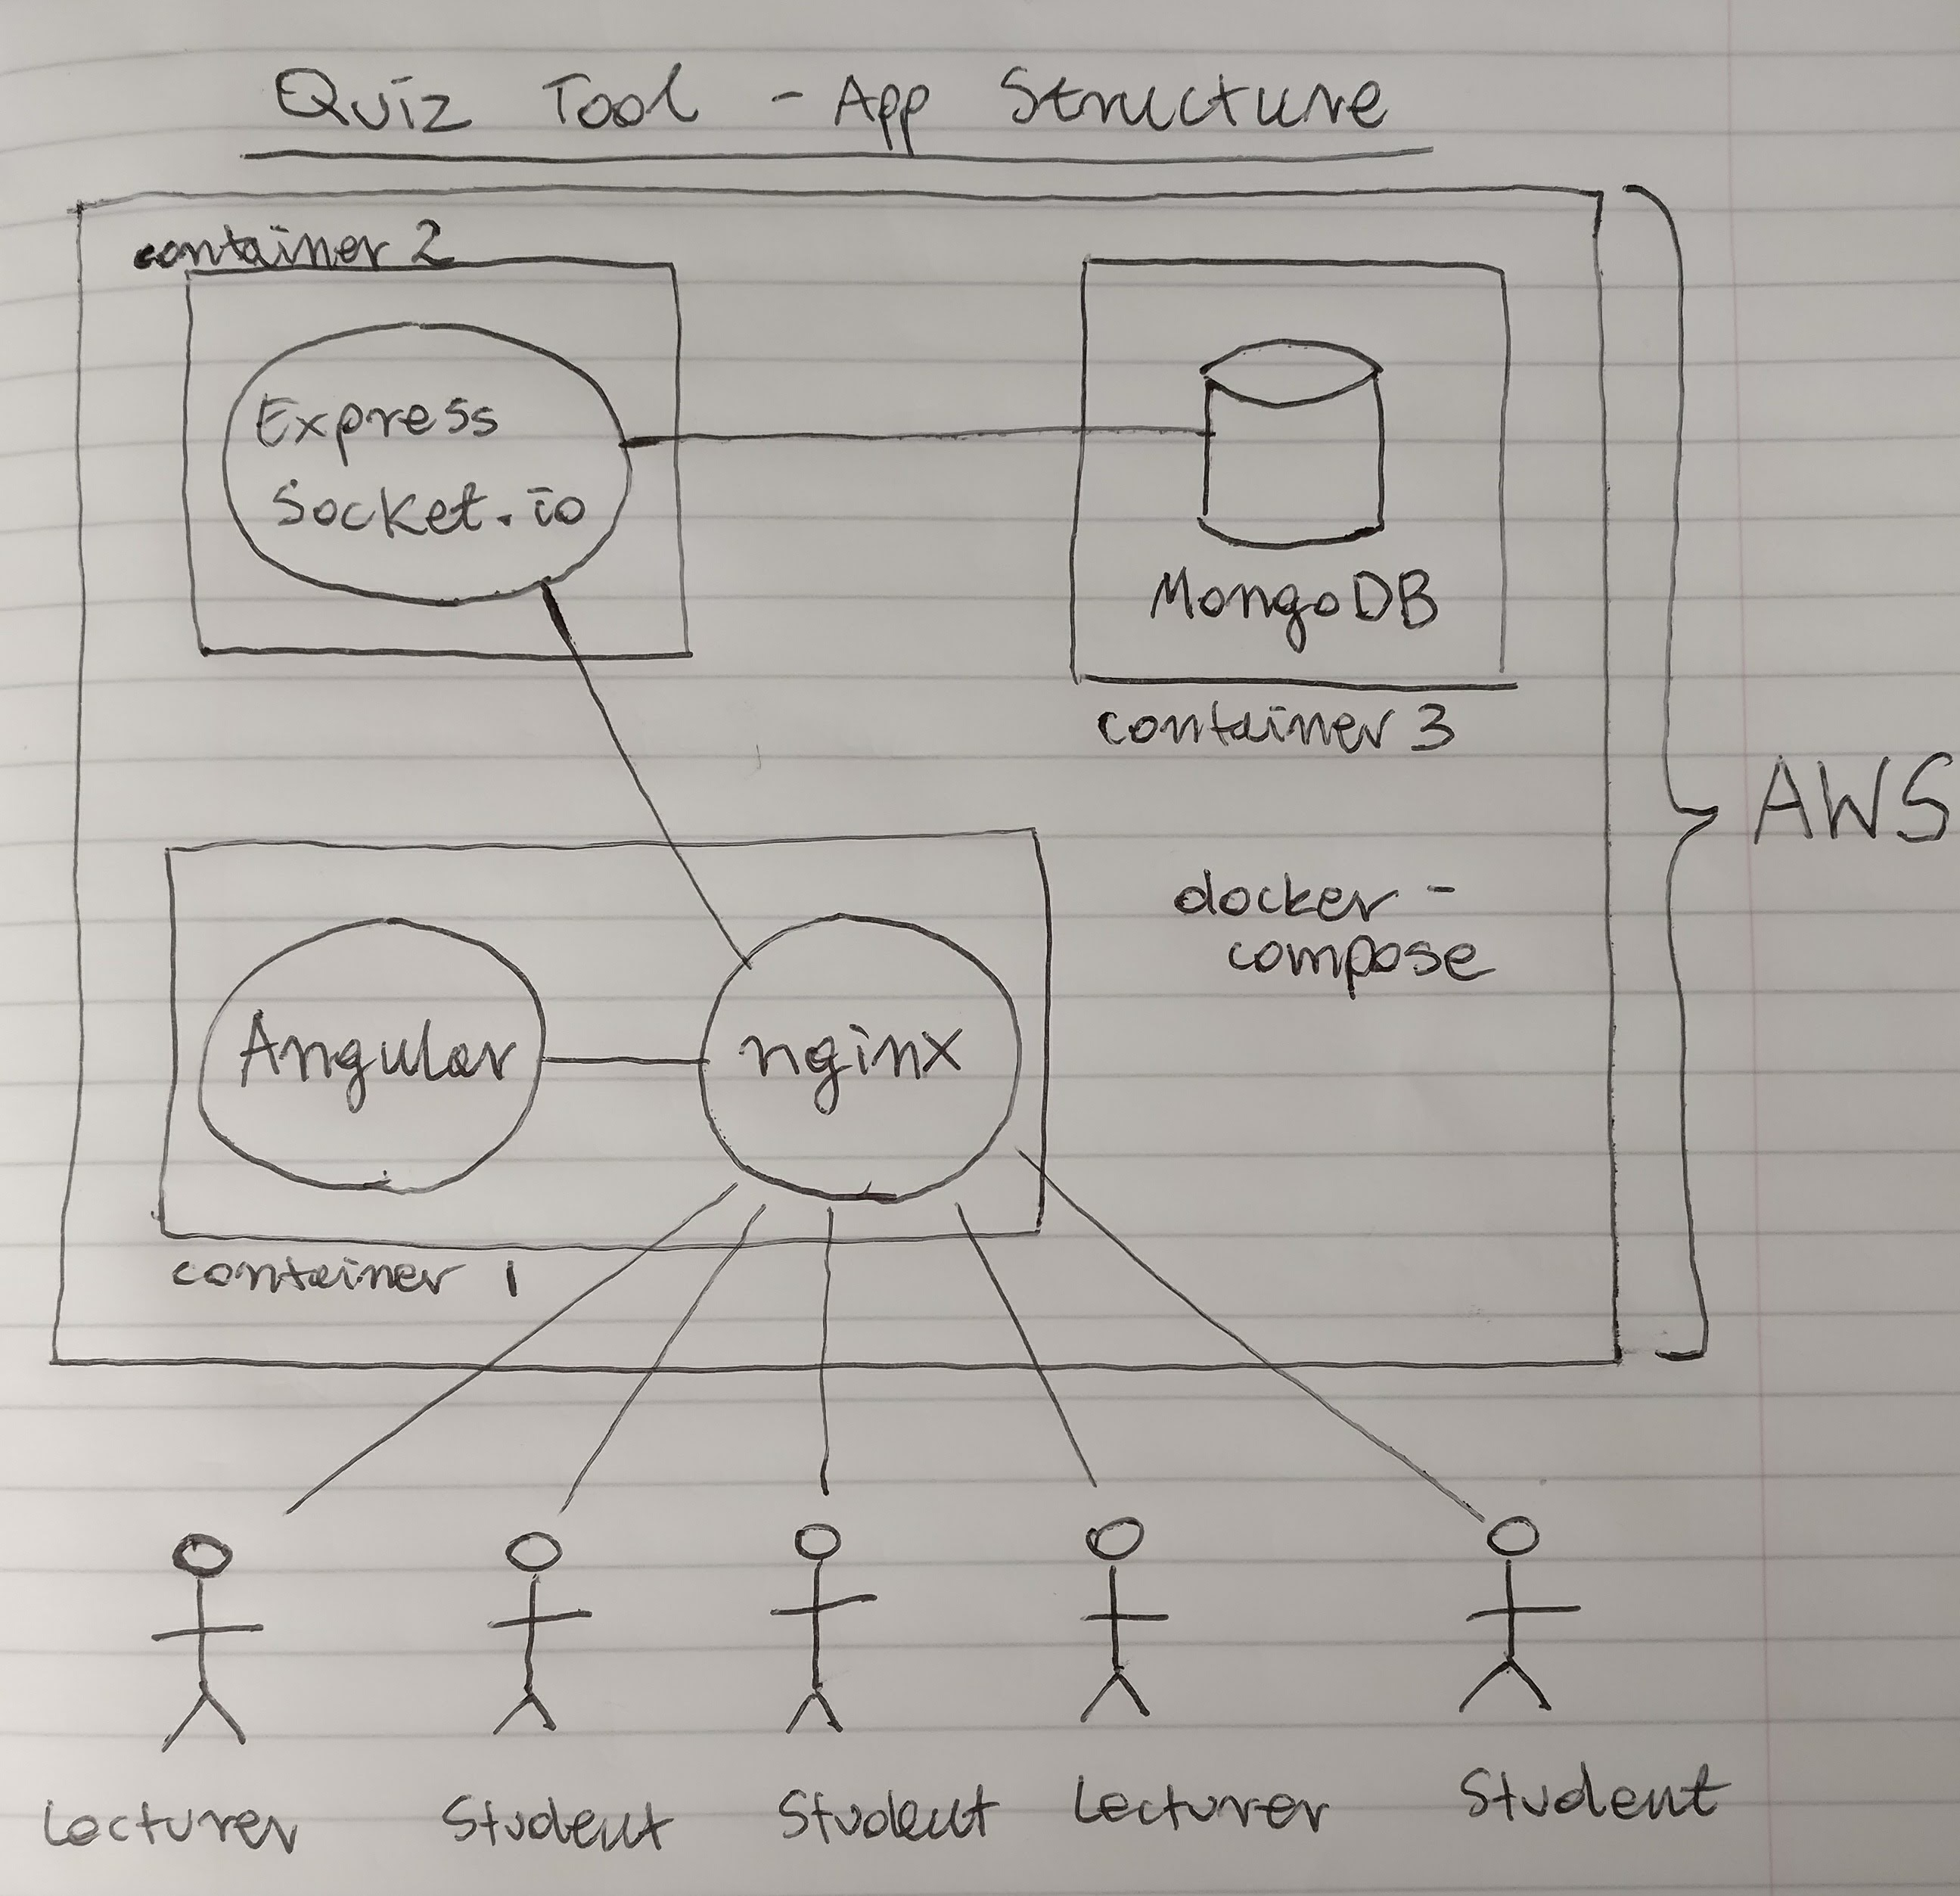
\includegraphics[width=0.7\textwidth]{../../design/app_structure.jpg}
    \caption{The proof of concept application structure}
    \label{fig:appstrucure}
\end{figure}

\begin{figure}[h!]
  \begin{lstlisting}[basicstyle=\small]
  version: '2.0'
  services:
    client:
      build: client
      ports:
        - "80:80"
      links:
        - server_node
    server_node:
      build: server
      links:
        - database
    database:
      image: mongo
      ports:
        - "27017:27017"
  \end{lstlisting}
  \caption{The docker-compose.yml file describing the tool's structure}
\end{figure}

\newpage
\subsubsection{Front End Container}
The front end container consisted of Angular 4 and nginx reverse proxy. The structure
has been based on the \textit{Dockerized Angular 4 App (with Angular CLI)} repository\cite{35}.
The Socket.io client dependency has been added to allow sending messages to the back end
using sockets. The initial \texttt{Dockerfile} included in the \autoref{chap:codesamples} of this report
as the \autoref{sample:clientdocker} uses the multi-stage build added in Docker 17.05. The
Angular app is compiled to JavaScript and HTML files during the initial stage of the build,
and then these files are copied to the nginx public folder to be served to clients.
This results in a lean, production ready image.

\subsubsection{Back End Container}
The back end container included in the \autoref{chap:codesamples} of this report
as the \autoref{sample:serverdocker} consisted of a Node.js runtime, the Express framework and the Socket.io
engine capable of pushing messages to clients using Sockets. The \texttt{Dockerfile} illustrates
the very basic Node container.

\subsubsection{Database Container}
Finally, the MongoDB Docker image has been pulled automatically from the official mongo
Docker Hub registry\cite{36}.

\subsection{Continuous Integration}
Circle CI has been integrated with the GitHub repository containing the source code of the
Quiz Tool. Every time a pull request was made, Circle CI would be notified. It would then
assign a virtual machine build agent from a pool, and spin up a clean build environment.
It would then checkout the code and run the steps specified in the build config file, before
reporting if the build was successfull back to GitHub.

\begin{figure}[ht]
    \centering
    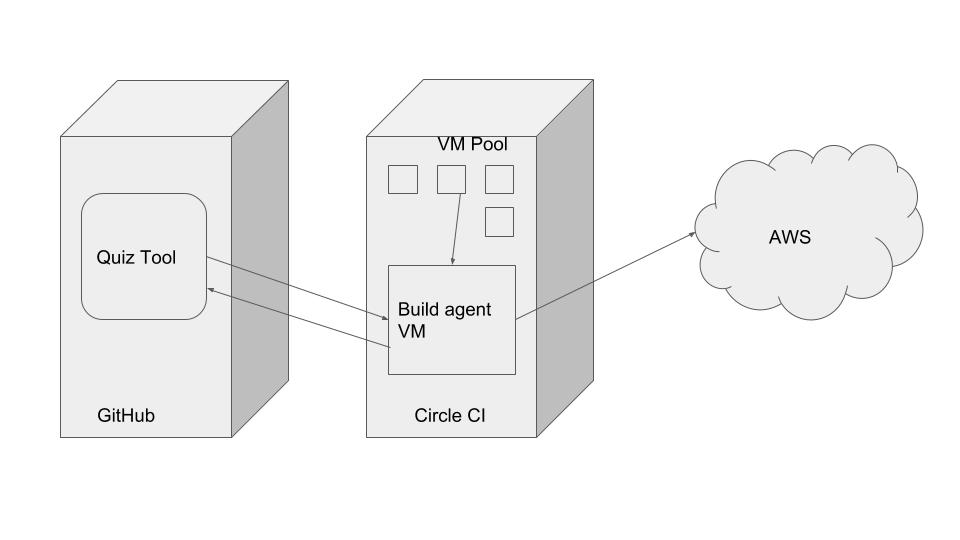
\includegraphics[width=0.8\textwidth]{circleci.jpg}
    \caption{Continuous Integration and Deployment}
    \label{fig:ci}
\end{figure}

The \texttt{.circleci/config.yml} file included in the \autoref{chap:codesamples} of this report
as the \autoref{sample:circleci}, describes the initial build steps of the Quiz Tool.
Code is checked out from the version control, all the dependencies necessary to perform following
steps are installed, the project is then built and started using docker-compose, before the
\texttt{curl localhost} command checks if the application is up and running. Finally, if
the current branch being built is \texttt{master}, the \texttt{deploy.sh} bash script runs, which
deploys the application to production.

\subsection{Production Environment}
The production environment of the tool is hosted on the AWS cloud. The AWS Elastic Beanstalk
has been chosen specificaly, as applications in
various programming languages can be deployed with ease, wihout having to worry about
the infrastructure running these applications\cite{37}. The Multicontainer Docker AWS Elastic
Beanstalk\cite{38} environment, creates a single Amazon EC2\cite{39}
instance and uses ECS (Amazon Elastic Container Service)\cite{40} to coordinate container deployments to
multicontainer Docker environments. The similarity with docker-compose, means the Quiz Tool
would behave similarly on developer's machine, in testing and in production.

\begin{figure}[h!]
    \centering
    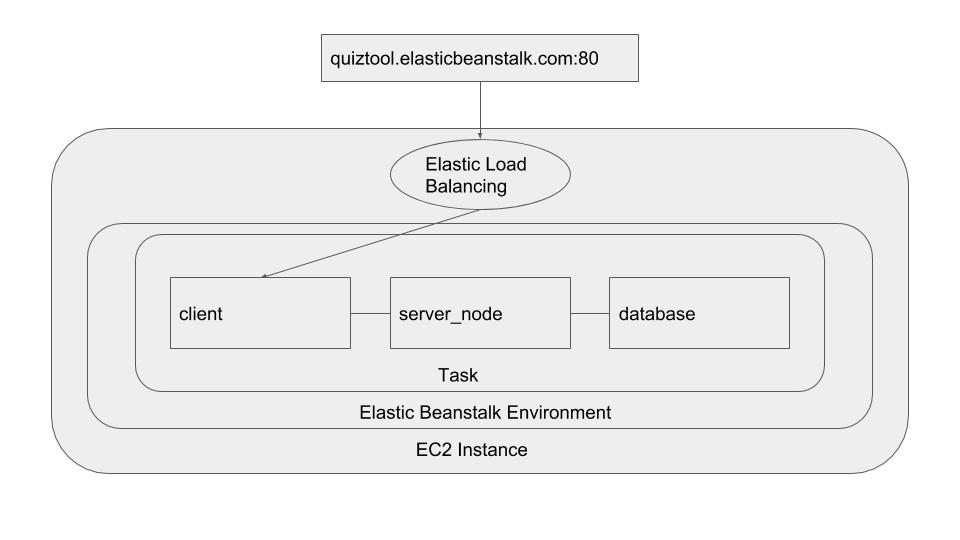
\includegraphics[width=0.8\textwidth]{elasticbeanstalk.jpg}
    \caption{Quiz Tool Production Environment}
    \label{fig:ebs}
\end{figure}

\texttt{docker-compose.yml} files define how docker-compose should run Docker containers together.
\texttt{Dockerrun.aws.json} is the equivalent configuration file to specify relationships between Docker
containers running in the Multicontainer Elastic Beanstalk environment. The format of the config file
included in the \autoref{chap:codesamples} of this report
as the \autoref{sample:dockerrunaws} is very
similar to the docker-compose configuration files. The major
difference is that the AWS Elastic Beanstalk does not build Docker images itself, and images have
to be pulled dynamically from Docker registries. Docker registries are simply servers used for storage and
distribution of Docker images.

\subsubsection{Circle CI and AWS Integration}
The build agent automatically deploys the tool to production when the \texttt{master}
branch is being built. The bash script included in the \autoref{chap:codesamples} of this report
as the \autoref{sample:deploy} performs the actual deployment, and the
approach is based on the examples\cite{41}\cite{42}.
The \texttt{\$AWS\_ACCESS\_KEY\_ID} and the \texttt{\$AWS\_SECRET\_ACCESS\_KEY} environment
variables have been added to the build configuration using the Circle CI web panel.
The integration has been achieved by creating an AWS profile config file and installing
the \texttt{awsebcli} Elastic Beanstalk command line utility as one of the build steps.
Both \texttt{client} and \texttt{server\_node} containers are then tagged and pushed
to the private Docker image registry provided by Amazon Elastic Container Service, before
the \texttt{eb deploy prod-env} command actually triggers the production deployment.
Both front and back end containers are then pulled from the private registry specified
in the \texttt{Dockerrun.aws.json} file, while the mongo image is pulled directly from
the official mongo Docker hub.

\begin{figure}[h!]
    \centering
    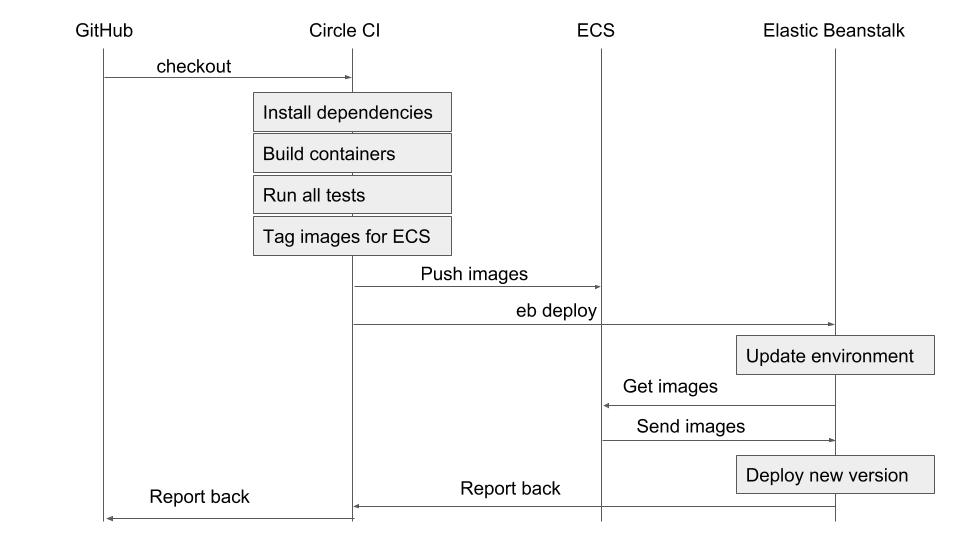
\includegraphics[width=0.8\textwidth]{deployment.jpg}
    \caption{Production Deployment Visualised}
    \label{fig:deploymentprocess}
\end{figure}

\subsection{Story Boards}
Including the customer
early in the development and design process allows teams to stay on track and readjust
their design if necessary. The story boards below have been produced to gain feedback
from the client, and ease the front end development in future iterations.

\autoref{fig:storylecturer} shows how the lectuer would login into the tool using
Google Single Sign On. He could then upload his lecture slides using an action
button in the bottom right corner of the screen, be able to edit his slides and
mark certain slides as quizzes. A list of cards would be presented showing all
lectures belonging to the lecturer and he could broadcast them to his audience.
Subsequently, he could navigate through the slides and slides with embedded quizzes would
split the screen in half to show a bar chart with answers as they come in. Finally,
lecture would end once he clicks the end button.

\autoref{fig:storystudent} on the other hand, shows how students could interact with
the tool. Student could join an ongoing lecture using a session key provided by the
lecturer. She could then participate in the lecture by watching the slides, and
submitting answers to quizzes as they come in. The correct answer could be presented
back to her in a form of a bar chart.

\begin{figure}[h!]
    \centering
    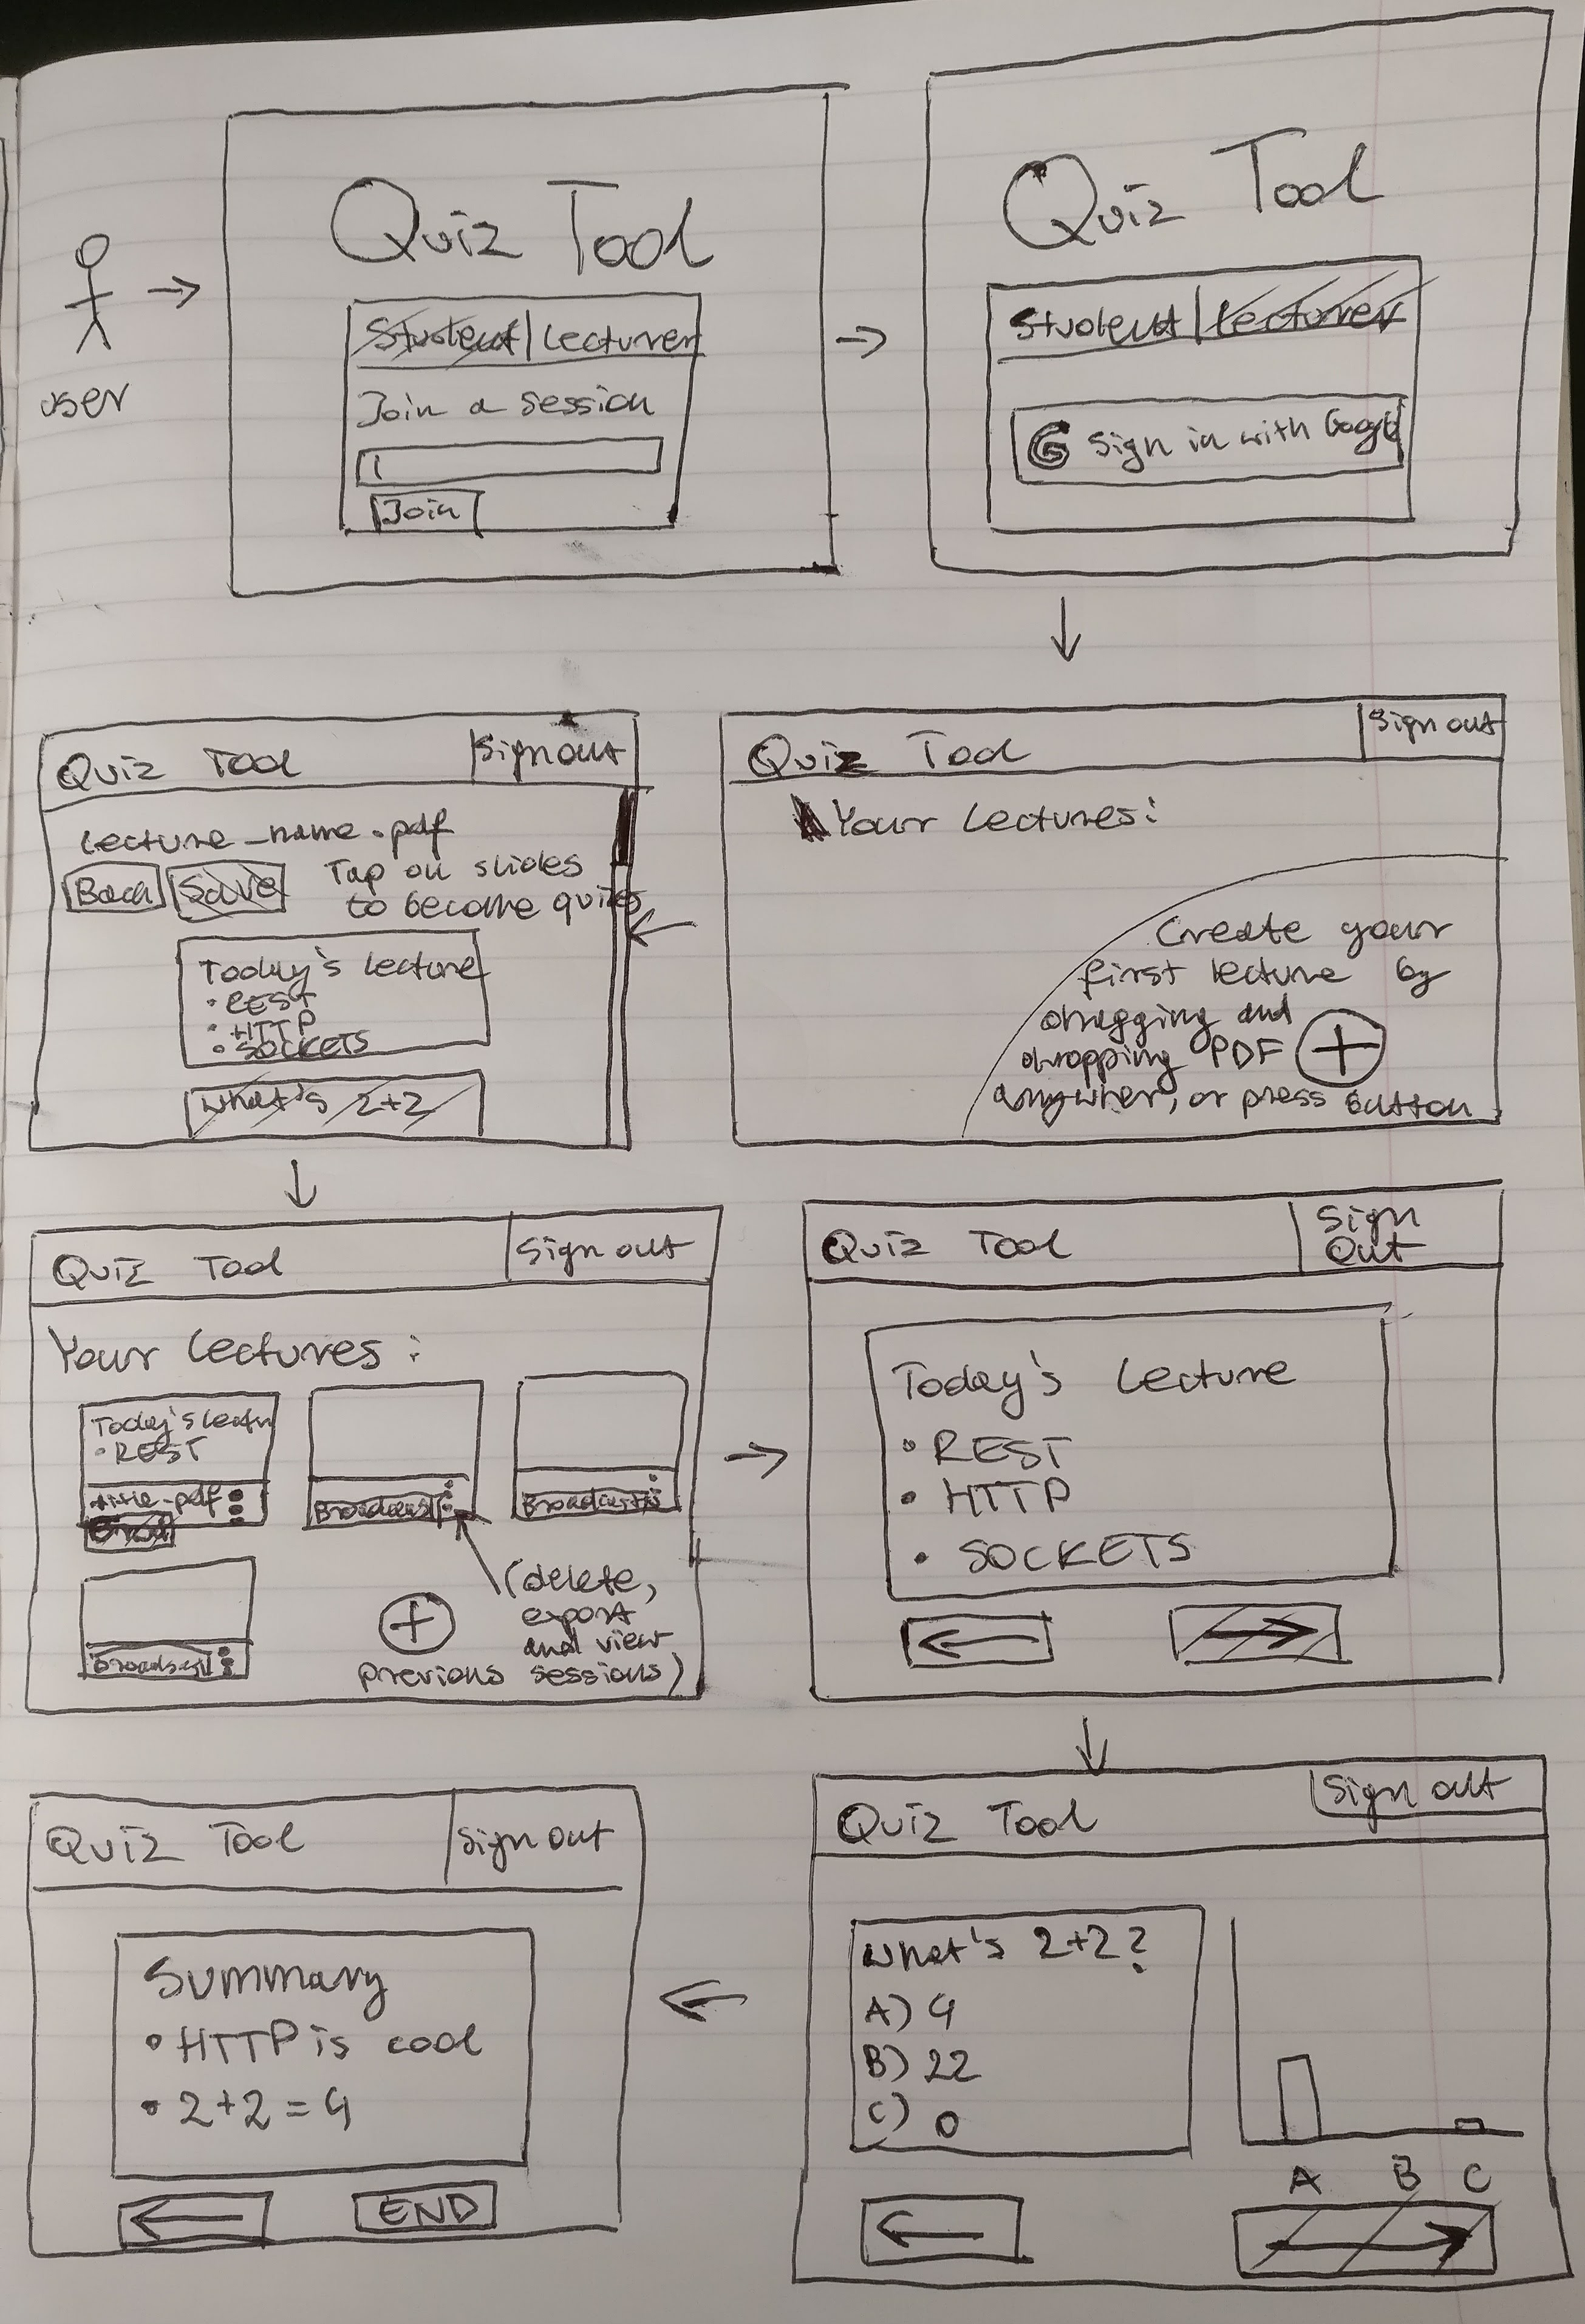
\includegraphics[width=0.9\textwidth]{../../design/story_board_lecturer.jpg}
    \caption{Story Board Lecturer Interaction}
    \label{fig:storylecturer}
\end{figure}

\begin{figure}[ht]
    \centering
    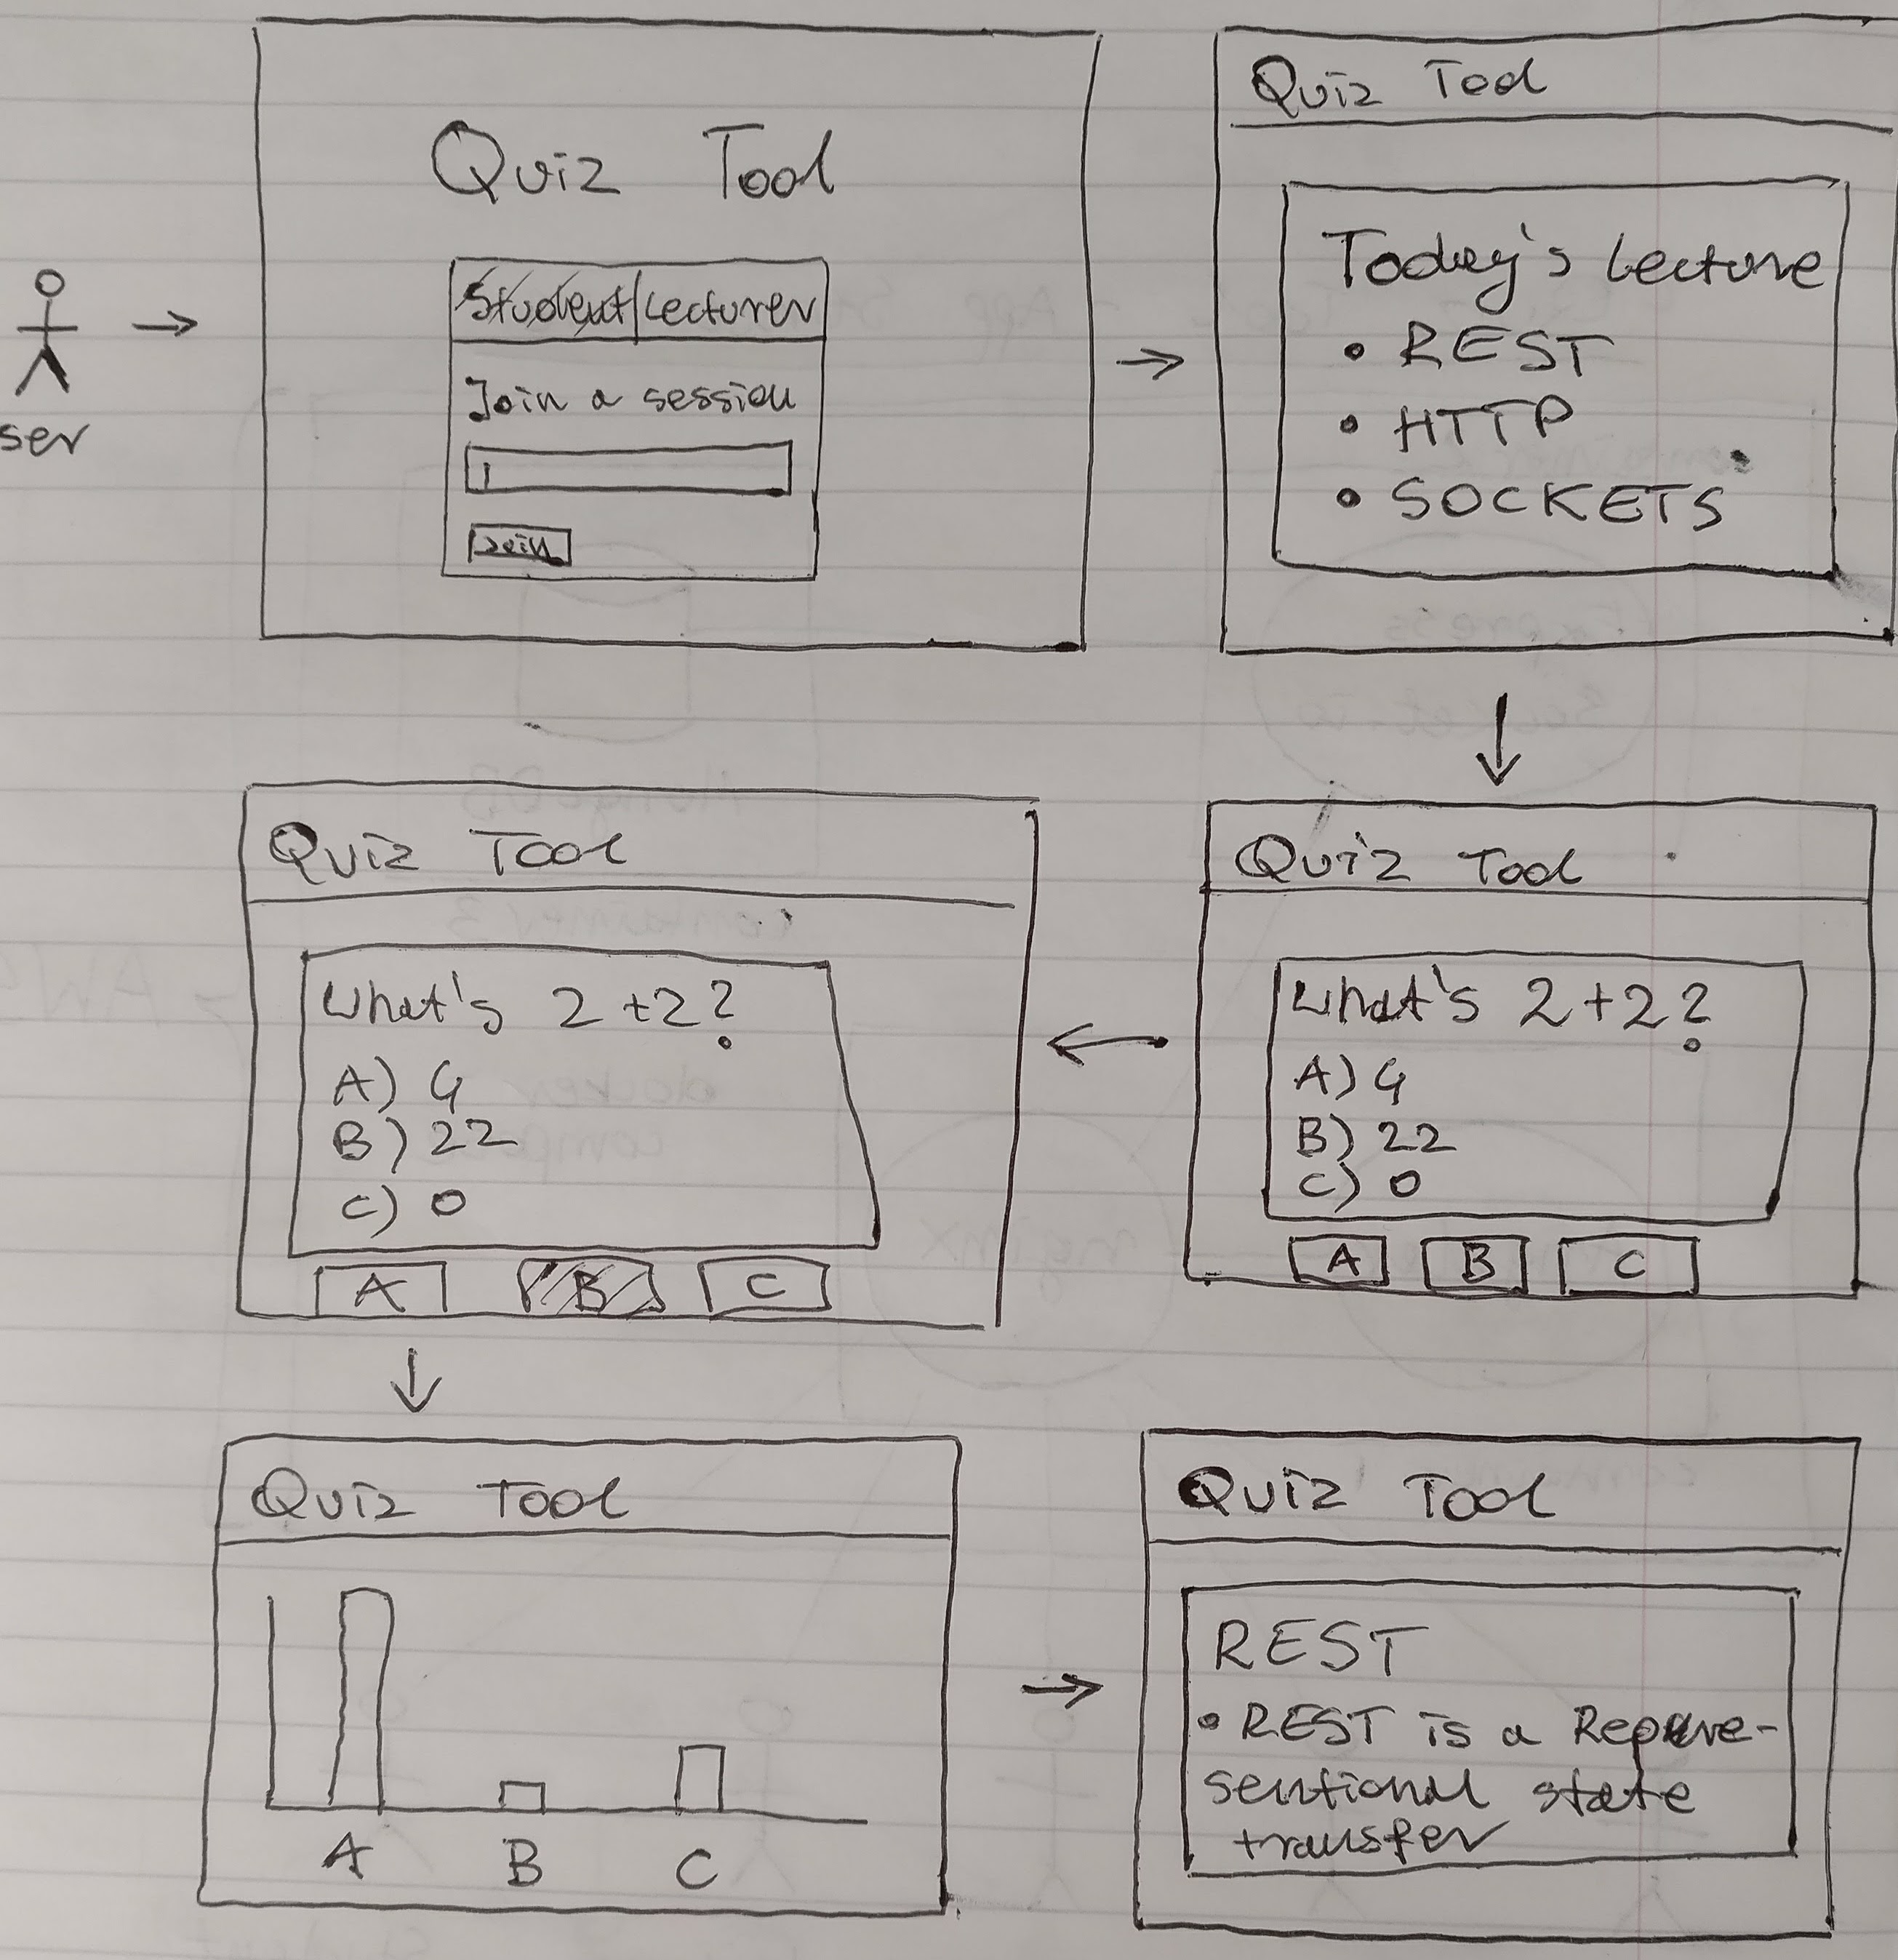
\includegraphics[width=0.9\textwidth]{../../design/story_board_student.jpg}
    \caption{Story Board Student Interaction}
    \label{fig:storystudent}
\end{figure}

\newpage
\subsection{Sprint Retrospective}
The first sprint proved it was possible to deploy a MEAN stack, containerised application
to production using Circle CI. Crucial DevOps has been successfully put in place, and the
initial feedback has been gathered from the client thanks to the low fidelity prototypes.
The full sprint retrospective document produced can be found in the \autoref{chap:spintretrospectives} of this report.

\begin{figure}[ht]
    \centering
    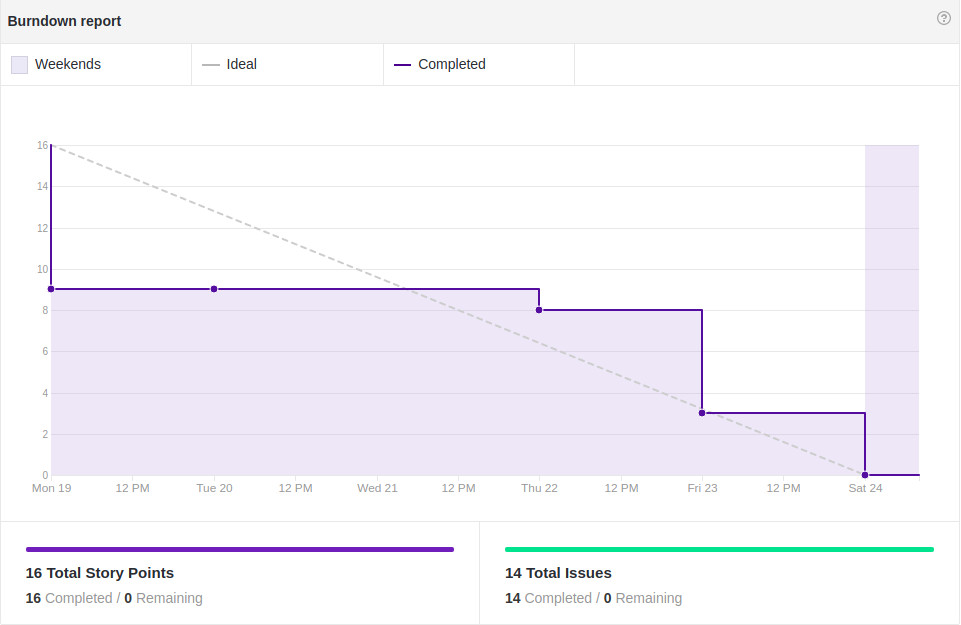
\includegraphics[width=\textwidth]{burn1.jpg}
    \caption{Burndown Chart Sprint 1}
    \label{fig:burn1}
\end{figure}

\newpage
\section{Sprint 2 - Bare Bone Application}
\subsection{Sprint Planning}
This sprint focused on converting the proof of concept chat application created in the previous
week into a basic Quiz Tool. Simple login page for both students and lectuers
would be developed based on the paper prototypes from the previous sprint, and Google Single Sign
On would be added. Once logged in, lectuers could upload their PDF lecture slides and broadcast
them to all students, as session generation was not implemented yet. The entire list of estimated stories
can be found in the \autoref{chap:spintstories} of this report.

\newpage
\subsection{Login Page and Authorisation}
% - JWT tokens
% - JWT interceptor
% - Google single sign on
% - session cookies
The login page has been created based on the low fidelity prototypes, and allowed
lecturers to log into the tool, and students to join ongoing lectures with a session key.
The Materialize\cite{43} CSS framework has been added to achieve a modern user interface.

\begin{figure}[h!]
    \centering
    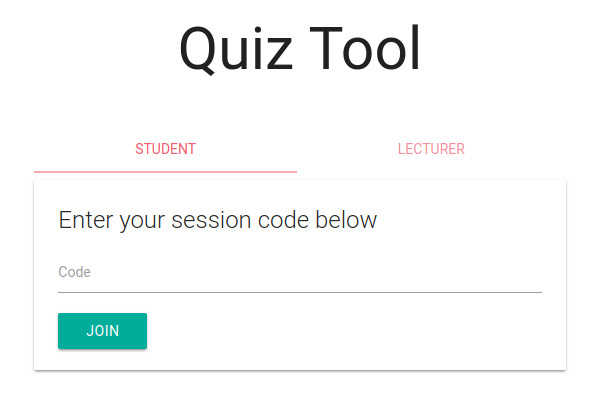
\includegraphics[width=0.8\textwidth]{student_login.jpg}
    \caption{Student Login Page}
    \label{fig:studentlogin}
\end{figure}

\begin{figure}[h!]
    \centering
    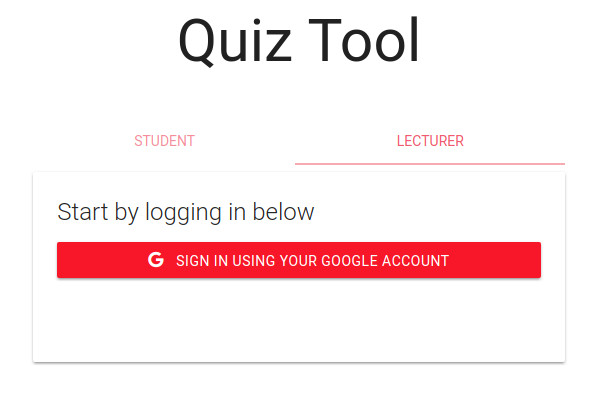
\includegraphics[width=0.8\textwidth]{lecturer_login.jpg}
    \caption{Lecturer Login Page}
    \label{fig:lecturerlogin}
\end{figure}

Angular has a concept of guards, which allow specified routes to be only accessible to
authorised users. The code extracted from the \texttt{client/src/app/app.routing.ts} below
shows how the desired behaviour has been achieved. All undefined routes redirect to the \texttt{/}
which has a \texttt{canActivate: [AuthGuard]} protection. The guard checks if the current user has a
valid session cookie with a JWT token\cite{44} present as described in the subsection below, before allowing
the user to navigate to his dashboard.

\begin{figure}[h!]
    \begin{lstlisting}[basicstyle=\small]
    const routes: Routes = [
      { path: '', component: DashboardComponent, canActivate: [AuthGuard] },
      { path: 'login', component: LoginComponent },
      { path: 'lecture/:code', component: LectureComponent },
      { path: '**', redirectTo: '' }
    ];
    \end{lstlisting}
    \caption{Angular Routing With Guards}
    \label{fig:auth}
\end{figure}

\subsubsection{Google Single Sign On and JWT Tokens}
Once the lecturer clicks on the Google Sign-In button, he is redirected to Google
and asked to provide his Google credentials, and authorise the Quiz Tool to get
basic information about him. The passport.js\cite{45} Node.js middleware, together
with the Google passport strategy\cite{46} have been added to handle the OAuth2\cite{47} authorisation.
Once the lecturer authorises Quiz Tool to get the basic information about him, Google calls the
\texttt{/auth/google/callback} callback defined in the \texttt{server/index.js}. The callback
handler located in the \texttt{server/helpers/passport.helper.js} takes the access token, user's
Google display name and his public Google ID, and stores them in the database by creating a new
lecturer entry in MongoDB. Finally, a session cookie is sent back to the lecturer's client
containing the access token.

As mentioned before, the \texttt{AuthGuard} on the Angular side makes sure user is logged in, before
rendering his dashboard. The guard uses the \texttt{client/src/app/services/auth.service.ts} to make
sure the session cookie exists. Each HTTP call Angular makes to the back end is intercepted by
the \texttt{client/src/app/utils/jwt.interceptor.ts} which checks if user has the token, and if so,
an extra authorisation header is added containing the token in the format \texttt{Authorization: Bearer fancyJSONToken123}.
Finally, all routes on the back end are protected with the \texttt{server/helper/auth.helper.js}, which
checks if the token provided exists in the database, is valid and has not expired, by checking with Google if it was issued
against the Quiz Tool.

\subsection{Persistence Layer}
MongoDB is a document storage, enabling persistence of JSON-like documents with extra metadata
including internal object ids. Mongoose\cite{48} is a popular MongoDB object modelling library which has
been integrated with the server side of the Quiz Tool. It removes the need to write boilerplate code and
allows developers to focus on getting things done quickly. Schemas describing objects have been created
and can be found in the \texttt{server/models} directory. They allow mongoose to validate data before
it is allowed to be persisted in the database. Even though mongo is not a relational database, an
entity relationship diagram depicted in the \autoref{fig:initialERD} has been created to make the design more concrete.

\begin{figure}[h!]
    \centering
    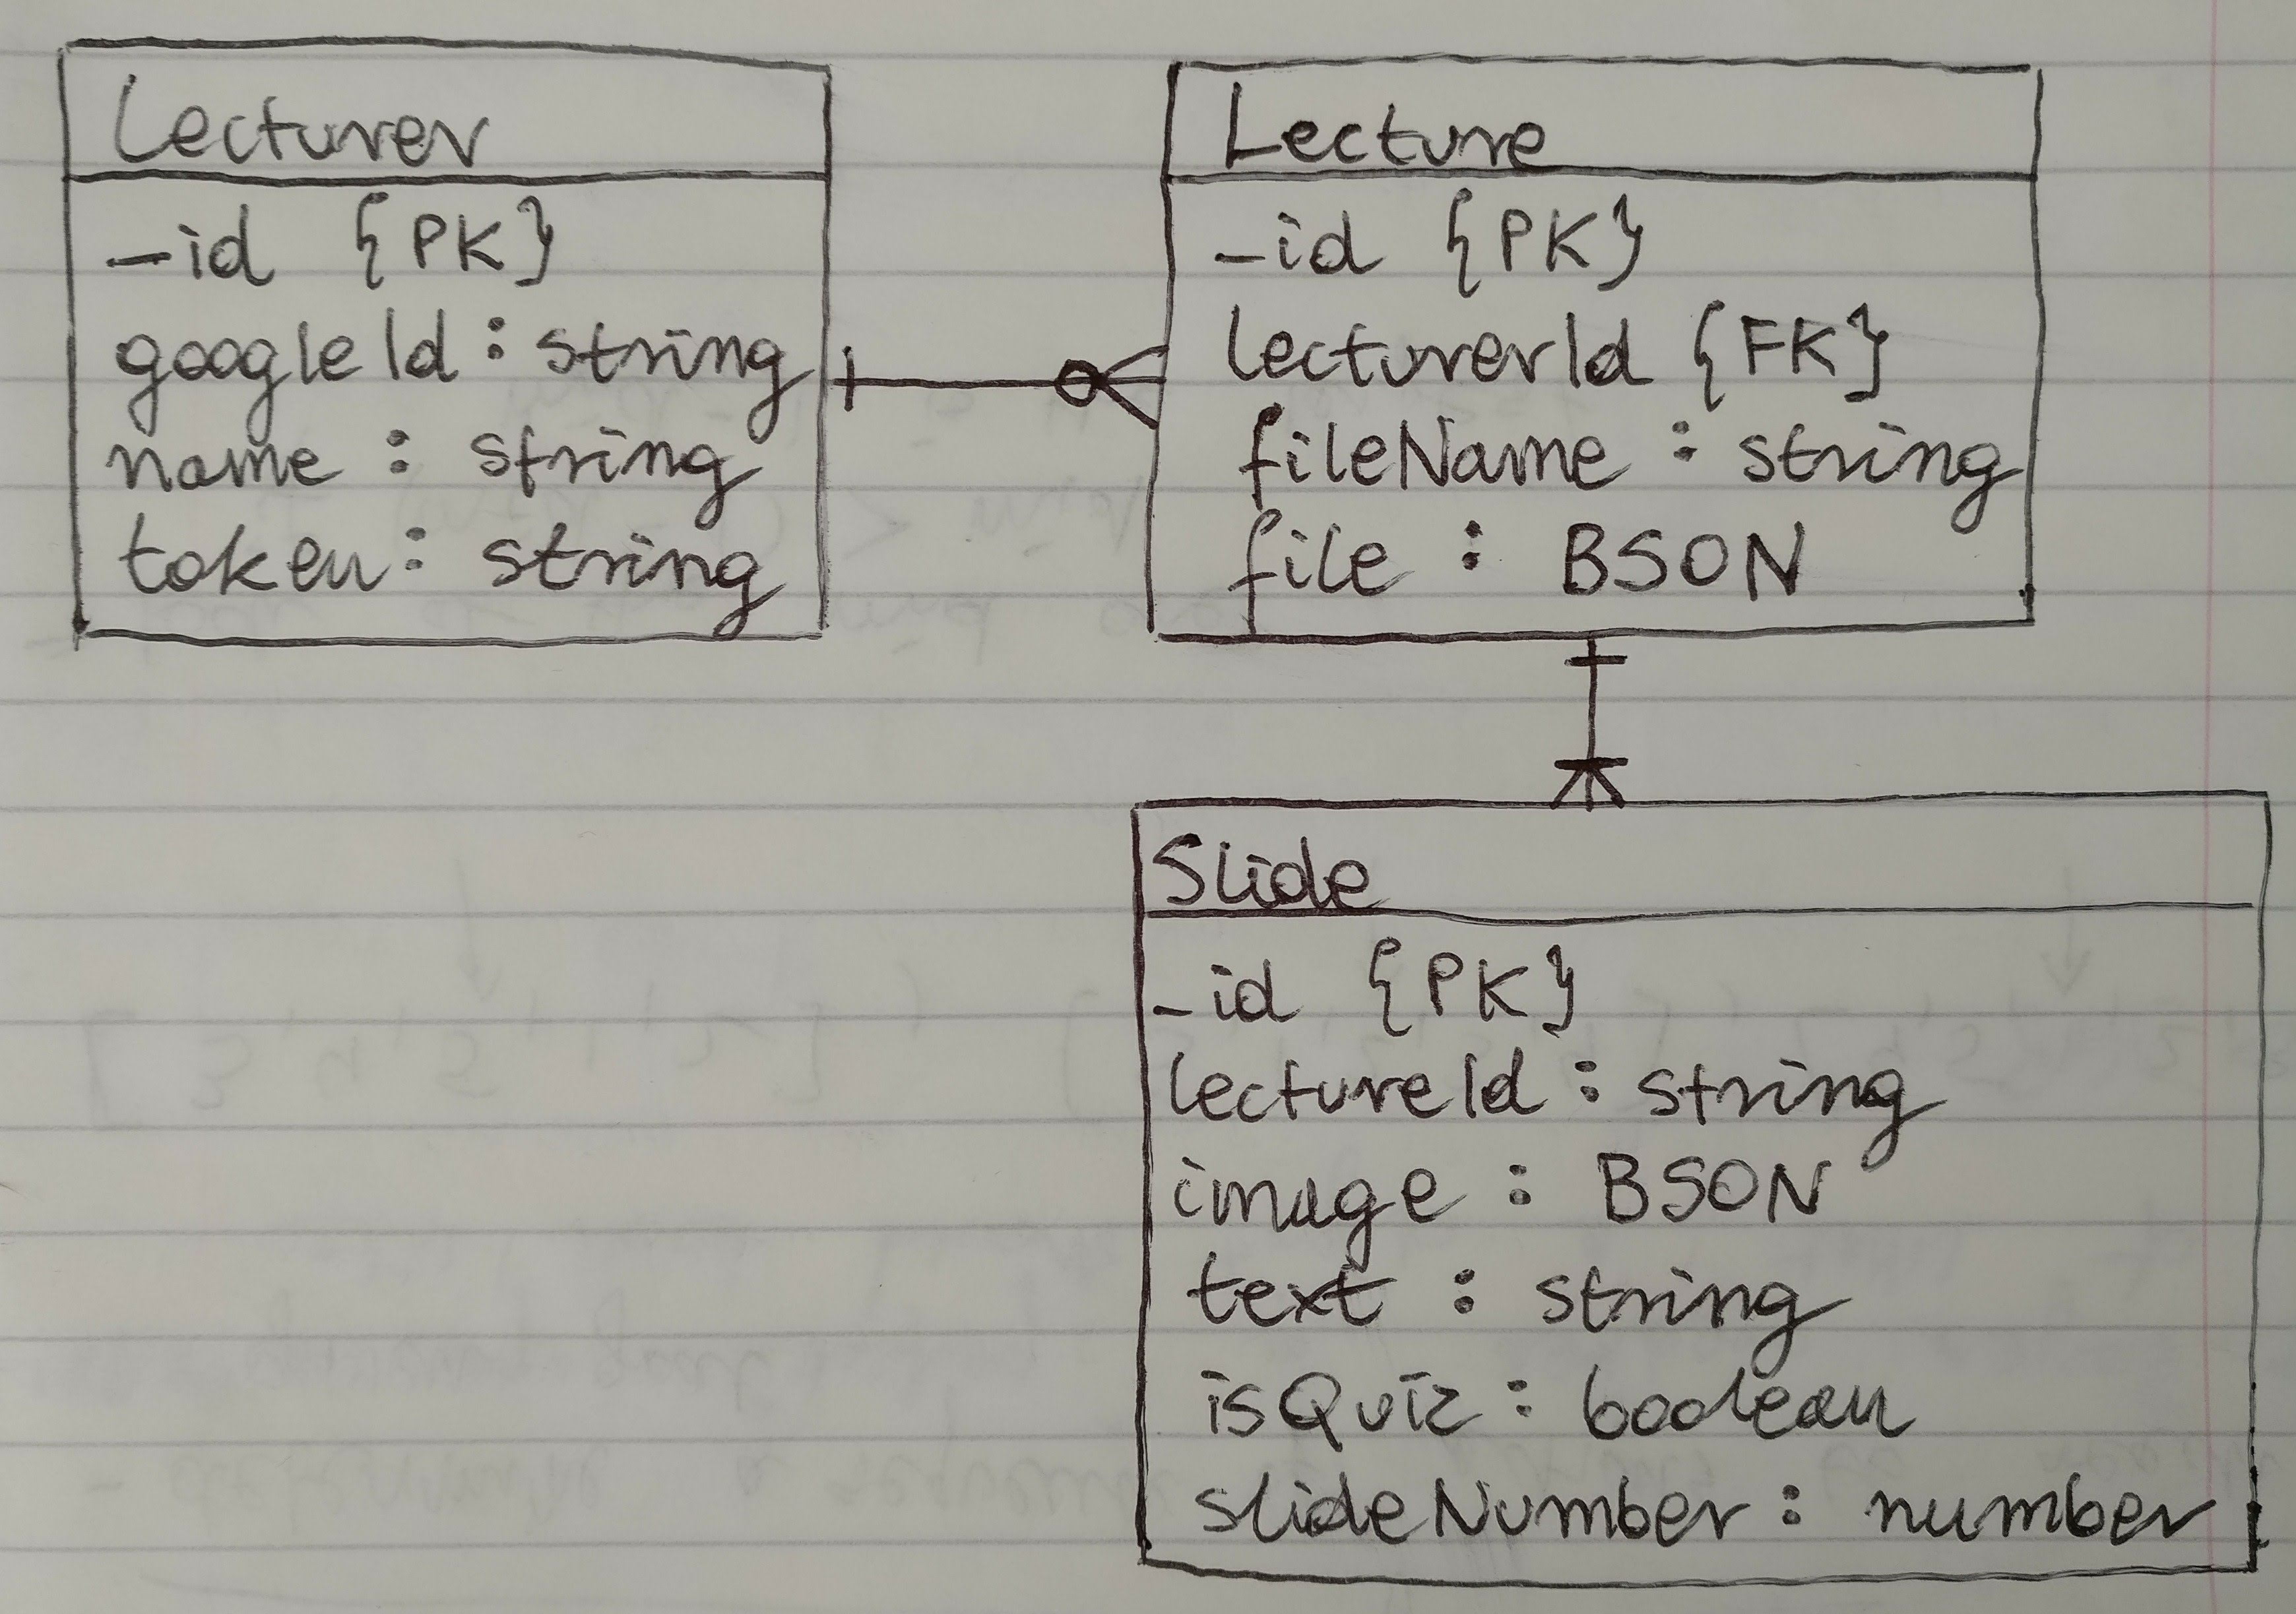
\includegraphics[width=0.8\textwidth]{initialERD.jpg}
    \caption{Initial Entity Relationship Diagram}
    \label{fig:initialERD}
\end{figure}

\subsection{Lecture Upload}

\begin{figure}[h!]
    \centering
    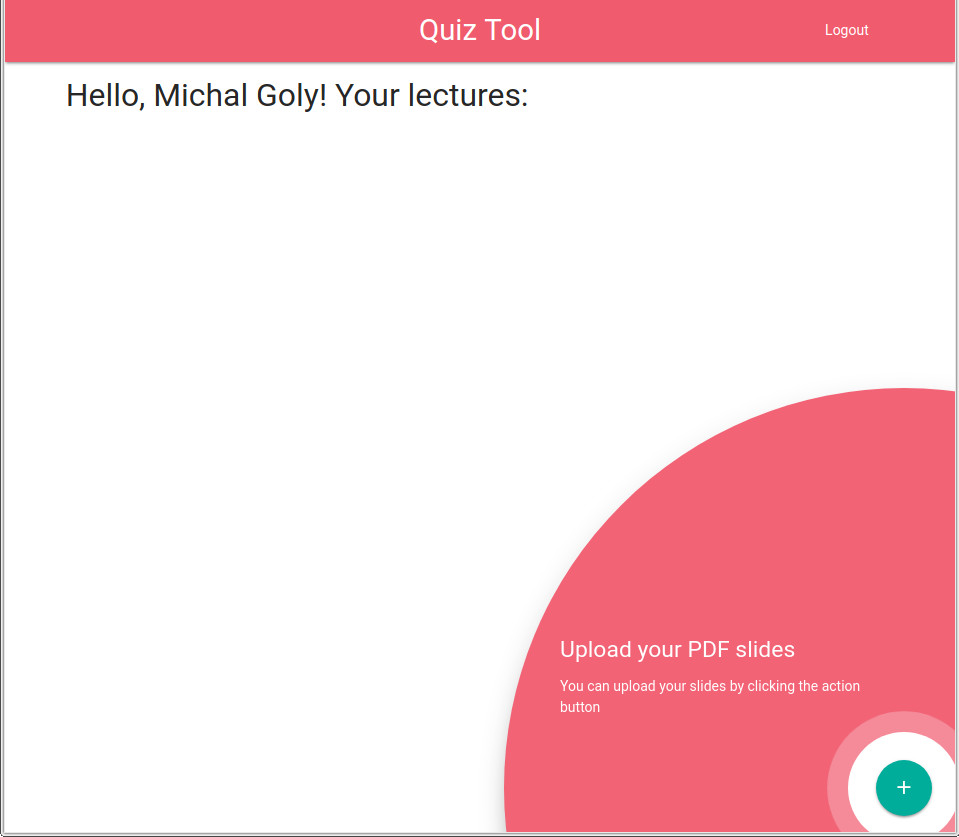
\includegraphics[width=0.8\textwidth]{dashboard.jpg}
    \caption{Dashboard View}
    \label{fig:dashboard}
\end{figure}

Once lecturer logs into the system he is presented with a dashboard view visible in the \autoref{fig:dashboard}.
The action button in the bottom right corner of the screen, allows PDF lecture slides to be uploaded.
The tool does not work with other presentation file formats for simplicity reasons. This could however
be extended in the future. Binary files can be stored in three major ways in MongoDB:

\begin{enumerate}
  \item Using the Mongoose BSON (Binary JSON)\cite{49} data type and setting it as type of a property of the document.
    This limits the file size to 16 MB.
  \item Using GridFS\cite{50} which relies on the client to have a driver capable of splitting the data into 255 KB
    chunks, and then streaming them into the database. This allows a binary file of any size to be persisted
    in MongoDB.
  \item Storing a file on an external storage, and persisting the reference to the file in the database.
\end{enumerate}

The BSON approach has been chosen for the Quiz Tool, as it significantly simplified the implementation and it is
unlikely PDF presentations over 16 MB would be commonly used. Again, this is something that could be changed
in the future if the lifespan of the tool extended beyond the final project submission.

\begin{figure}[h!]
    \centering
    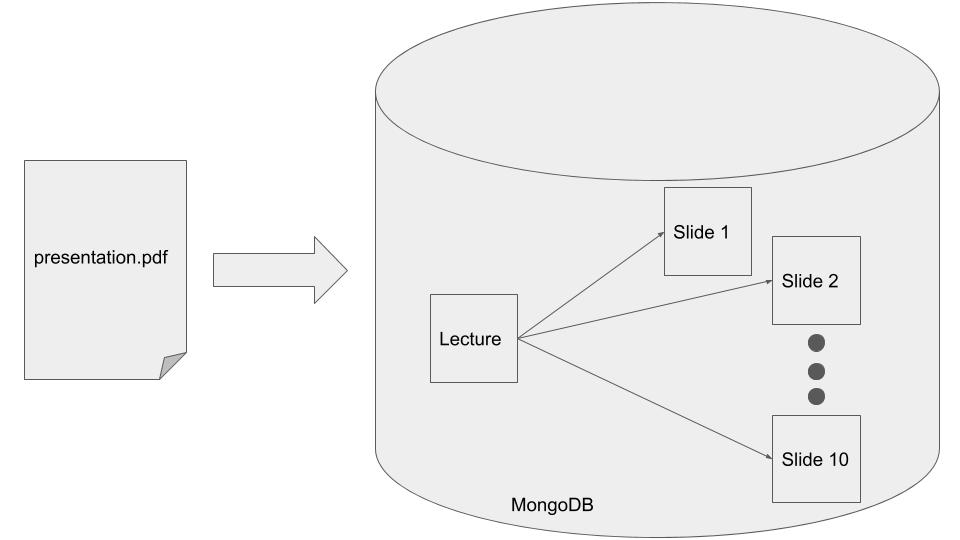
\includegraphics[width=0.8\textwidth]{fileupload.jpg}
    \caption{Initial File Upload}
    \label{fig:initialfileupload}
\end{figure}

The initial implementation of the file upload, took the PDF file, stored it directly as BSON in the
\texttt{Lecture} schema object and split the lecture into slides storing them in MongoDB using
the \texttt{Slide} schema object. Once the file has been uploaded using the ng2-file-upload\cite{51},
and persisted in the database, it has been stored temporarly on disk. Text would be extracted from
each slide using the pdf-extract\cite{52} library, which would be instructed to leave single paged
PDFs for each slide on disk. These PDFs would be then converted to PNG images using the scissors\cite{53}
library. Finally, slides' text and images would be grouped together and stored in MongoDB, before the
temporary files would be cleaned from disk.

\begin{figure}[ht]
    \centering
    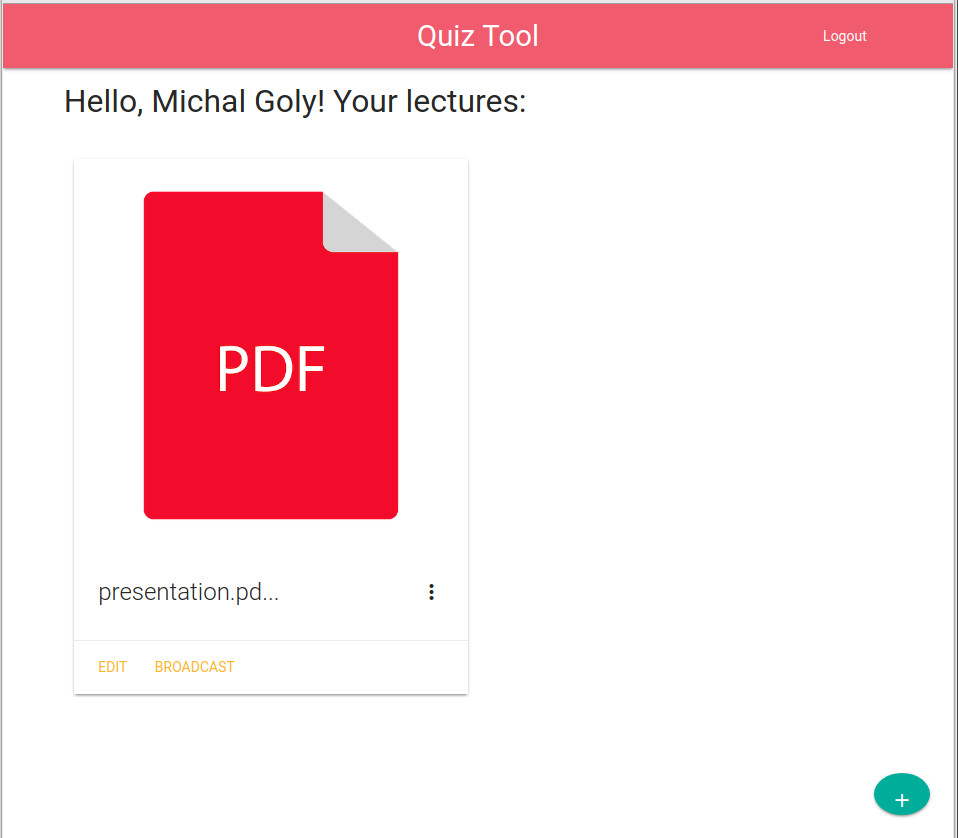
\includegraphics[width=0.8\textwidth]{dashboard_upload.jpg}
    \caption{Lecture Uploaded View}
    \label{fig:dashboarduploaded}
\end{figure}

\subsection{Lecture Broadcast}
\begin{figure}[h!]
    \centering
    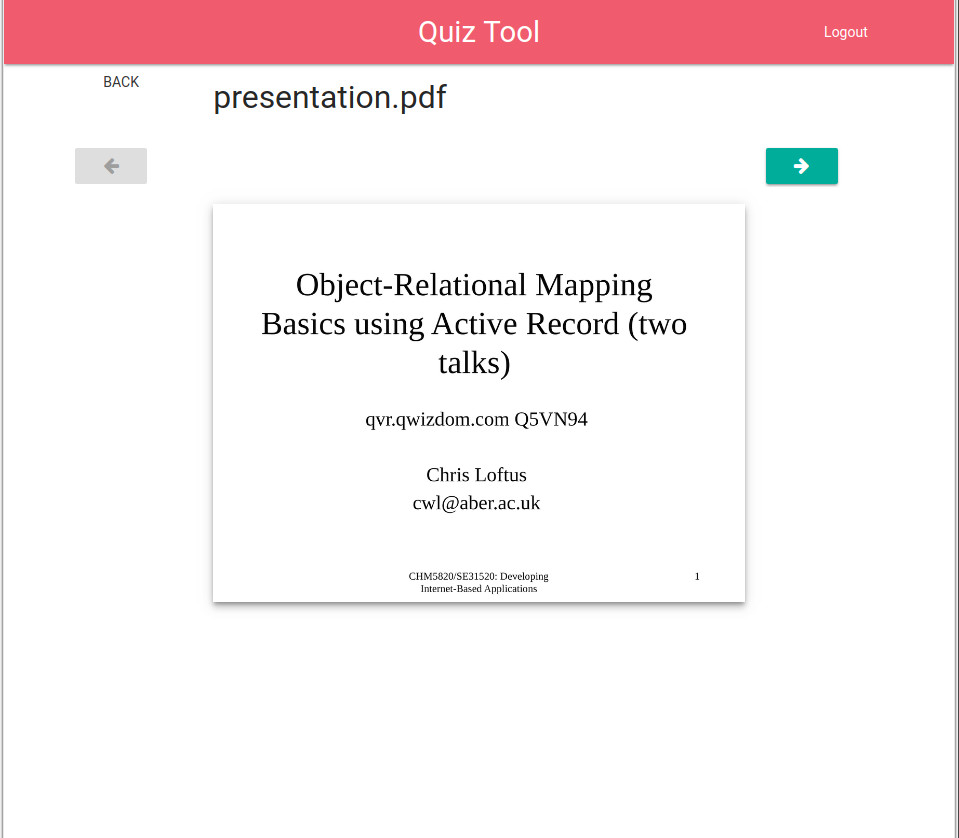
\includegraphics[width=0.8\textwidth]{broadcast.jpg}
    \caption{Initial Broadcast View}
    \label{fig:broadcast}
\end{figure}
Lectures could be broadcasted using the \textit{BROADCAST} action button located on the bottom
of each lecture card in the dashboard. \autoref{fig:broadcast} depicts the lecturer's view,
once the lecture starts. The initial implementation added in this sprint, did not have the
concept of a session yet, therefore slides were sent to all students who used any session key
to log into the tool.

Once the lecture was started, lecturer's client would pull all slides from the back end and emit the very
first one to all the students. Socket.io would be used to emit a simple event \textit{slide-change} containing
a JSON message in the following format: \texttt{\{"img": "base64img"\}}. PNG representations of each slide
were stored in the BSON format internally, but they were sent to clients using the Base64 binary-to-text format\cite{54}.
Students' clients would be then easily able to render such images using HTML \texttt{<img>} tags. Finally,
once the lecture was over, a \texttt{null} image would be sent to everyone and students' clients would
handle it by ending the lecture. The flow has been depicted in the \autoref{fig:sockets}.

\begin{figure}[h!]
    \centering
    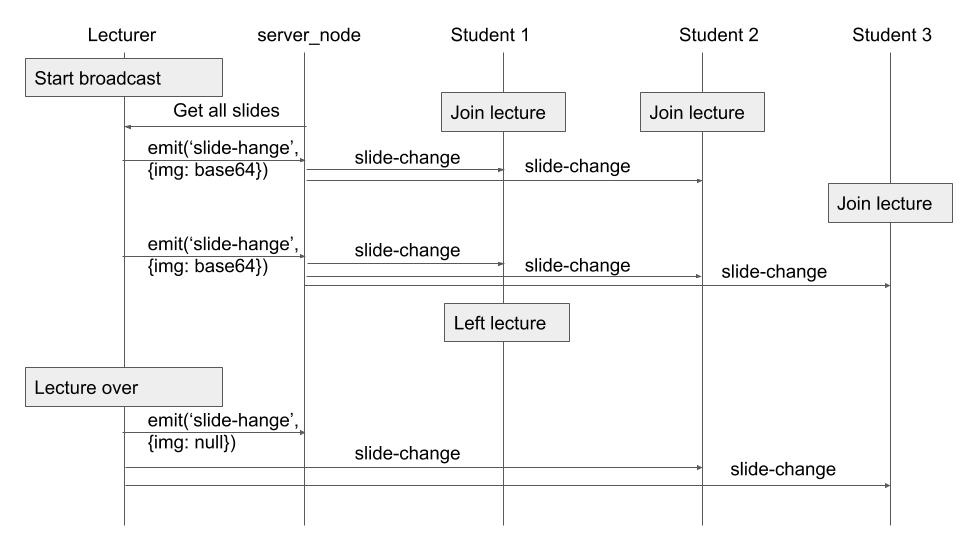
\includegraphics[width=\textwidth]{sockets.jpg}
    \caption{Initial Slide Broadcast Flow}
    \label{fig:sockets}
\end{figure}

\newpage
\subsection{Sprint Retrospective}
This was a very important sprint as it shaped the overall structure of the tool. The basis
of the Quiz Tool have been designed and implemented on both the front and the back end.
Schemas have been introduced to handle persistence, file uploads were implemented and
lecture slides could be emitted to all students using sockets in real time. The sprint
took two weeks, instead of one, as it was overfilled with too many issues.
The full sprint retrospective document produced can be found in the \autoref{chap:spintretrospectives} of this report.

\begin{figure}[h!]
    \centering
    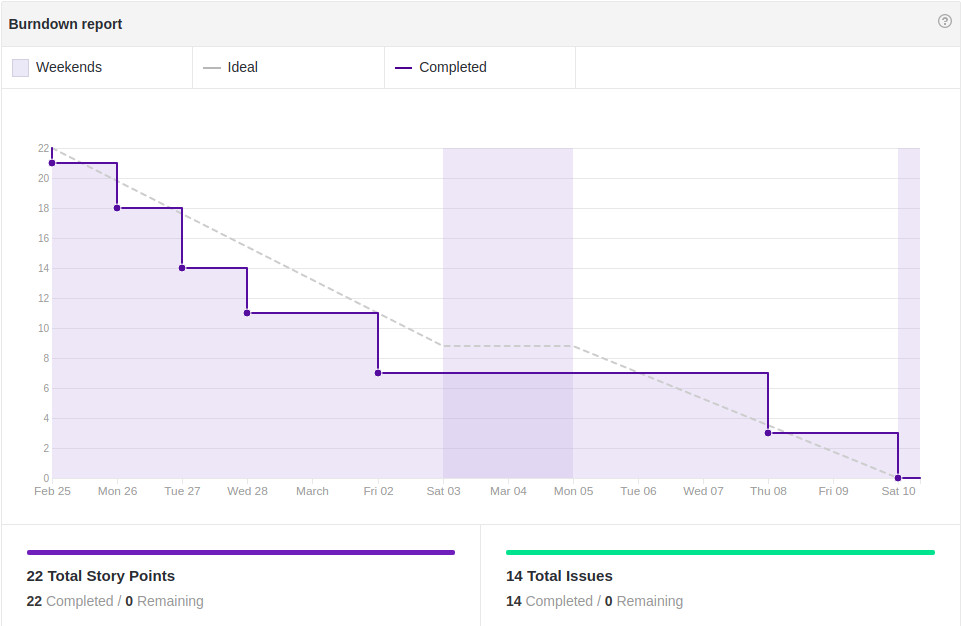
\includegraphics[width=\textwidth]{burn2.jpg}
    \caption{Burndown Chart Sprint 2}
    \label{fig:burn1}
\end{figure}

\section{Sprint 3 - Add Quizes}
\subsection{Sprint Planning}
This iteration focused on the ability to create quizzes, embed them into slides and
broadcast only to people who had the appropriate session key. The entire list of estimated stories
can be found in the \autoref{chap:spintstories} of this report.

\subsection{Session Keys}
Every time lecturer started a new broadcast, a random session code would be generated.
It would consist of eight alphanumerical characters, and the random generator would
be seeded with the current time, to decrease the probability of generating two idential
keys for two sessions running at the same time. The \textit{slide-change} Socket.io event
described in the previous sprint, has been extended to carry the appropriate session key
with each broadcast.

\begin{figure}[h!]
  \begin{lstlisting}[basicstyle=\small]
  {
    "img": "base64encodedImage",
    "sessionCode": "ABCD1234",
    "isQuiz": "false"
  }
  \end{lstlisting}
  \caption{The JSON Message Broadcasted on Slide Change}
\end{figure}

Students' clients are not uniquely identified by the Quiz Tool, therefore slides would
be broadcasted to all clients participating in the broadcast. Each client would
then know whether they have to update their \texttt{<img>} tag, by checking
if the session key entered by the student matches the key bundled with the image slide
arrived.

\subsection{Embedding Quizzes}
Each \texttt{Slide} in the system consisted of a PNG image and text extracted
from the PDF presentation uploaded by a lecturer. It also had a boolean flag
\texttt{isQuiz} specifying if given slide was supposed to be rendered as a quiz
or not. An edit panel visible below has been added, to allow lecturers to specify
which slides should be treated as quizzes.

\begin{figure}[h!]
    \centering
    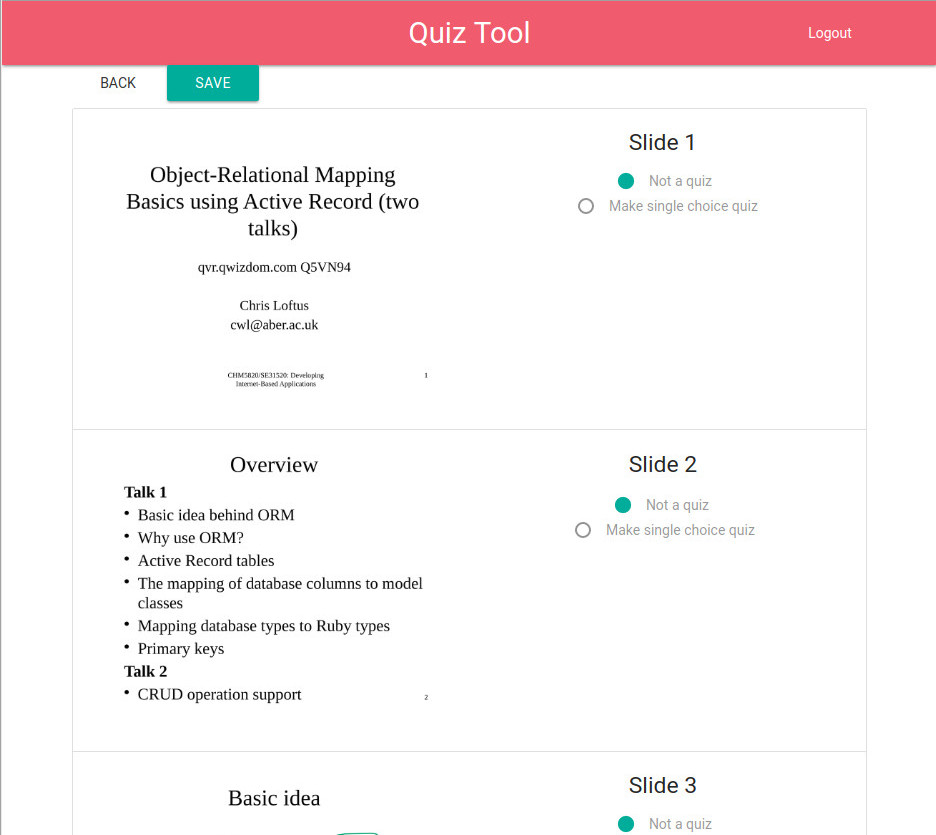
\includegraphics[width=0.8\textwidth]{editinitial.jpg}
    \caption{Initial Edit Page}
    \label{fig:editinitial}
\end{figure}

\newpage
\autoref{fig:editinitial} shows two radio buttons for each slide of a lecture.
These radio buttons could be used to mark certain slides as quizzes, by toggling
the boolean flag underneath. Text extracted from each slide would decide if a given
slide could become a quiz. If slide was not eligible to become a quiz, the radio button
to make it one would be greyed out. The initial implementation of the eligibility
algorithm checked if given slide contained at least two strings "A)" and "B)".
This was enough to make a slide eligible to be marked as a single choice quiz, and to be rendered as one,
as described in the next subsection.

\subsection{Quiz Rendering}
\autoref{fig:quizlecturer} shows the split screen view for a lecturer when a slide marked as a quiz was rendered
during a lecture broadcast. The left side shows the currently broadcasted slide, whereas the right
side shows a bar chart capable of displaying students' answers as they come in. Lecturer can
click the \textit{RETRY} button to wipe students' answers for current question and
ask again. Once he is happy with the results, he can select the correct answer which will
be shown to all people in the session, and then render the following slide, or even
the previous one if necessary. Students' answers were only stored in memory at this point
for the duration of the session.

\begin{figure}[h!]
    \centering
    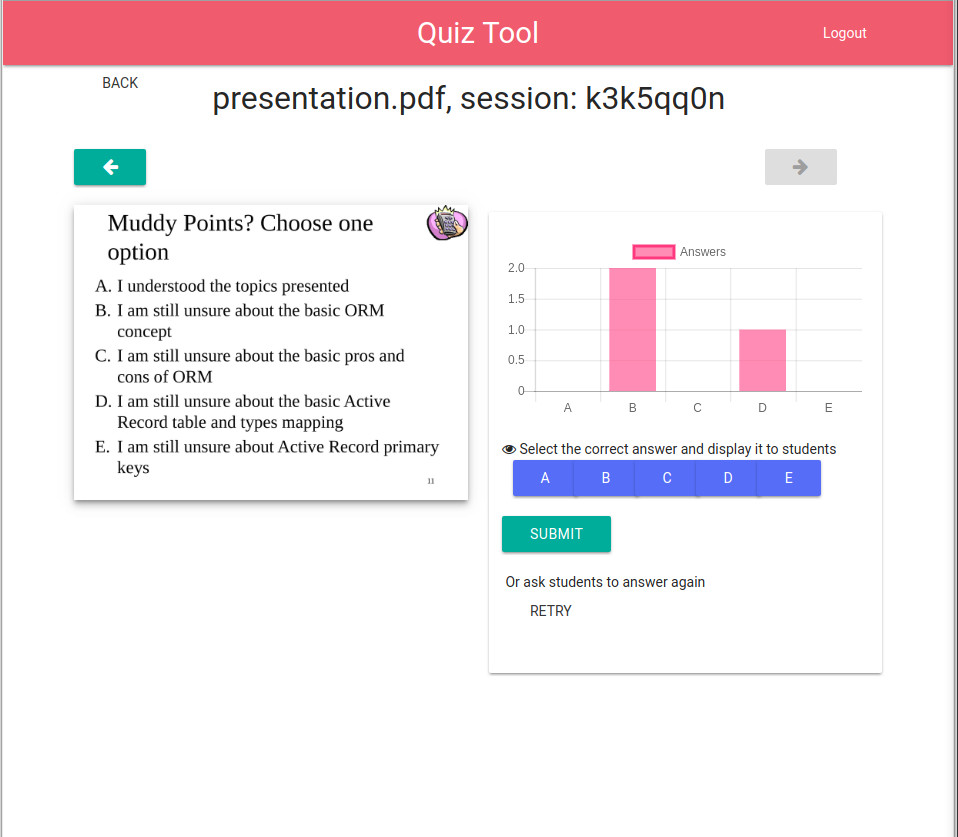
\includegraphics[width=0.8\textwidth]{quiz_lecturer.jpg}
    \caption{Quiz Rendering Lecturer}
    \label{fig:quizlecturer}
\end{figure}

\autoref{fig:quizstudent} on the other hand, shows the view rendered on students'
clients. They would be able to select one of the options and submit their answers
only once. The "A", "B", "C", "D", "E" buttons were generated automatically based
on the text of the slide. Students submitting their answers would emit an \textit{answer-received}
Socket.io event, bundled with a message in the format \texttt{\{"sessionCode": "ABCD1234", "option": "B"\}},
which would be then received by lecturer's client and rendered appropriately.

\begin{figure}[h!]
    \centering
    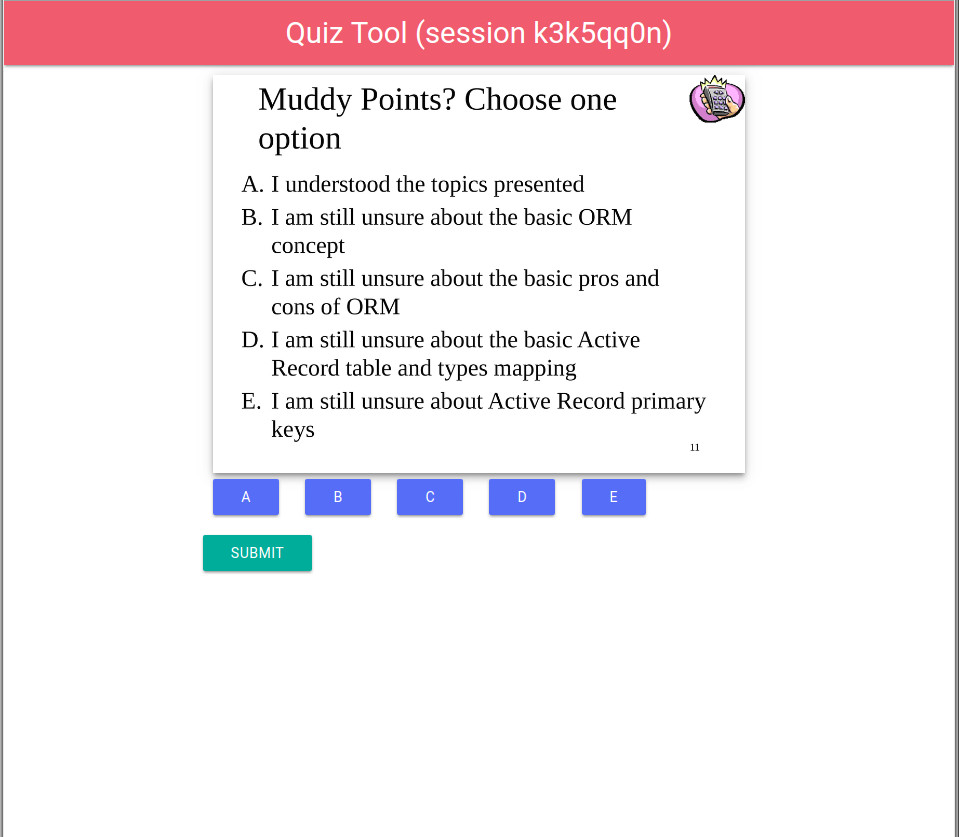
\includegraphics[width=0.8\textwidth]{quiz_student.jpg}
    \caption{Quiz Rendering Student}
    \label{fig:quizstudent}
\end{figure}

\subsection{Sprint Retrospective}
Following this iteration, Quiz Tool was able to handle quiz embedding which was a major
step towards the final implementation. Slides were no longer sent to everyone,
and multiple lectures could run at the same time.
The full sprint retrospective document produced can be found in the
\autoref{chap:spintretrospectives} of this report.

\begin{figure}[h!]
    \centering
    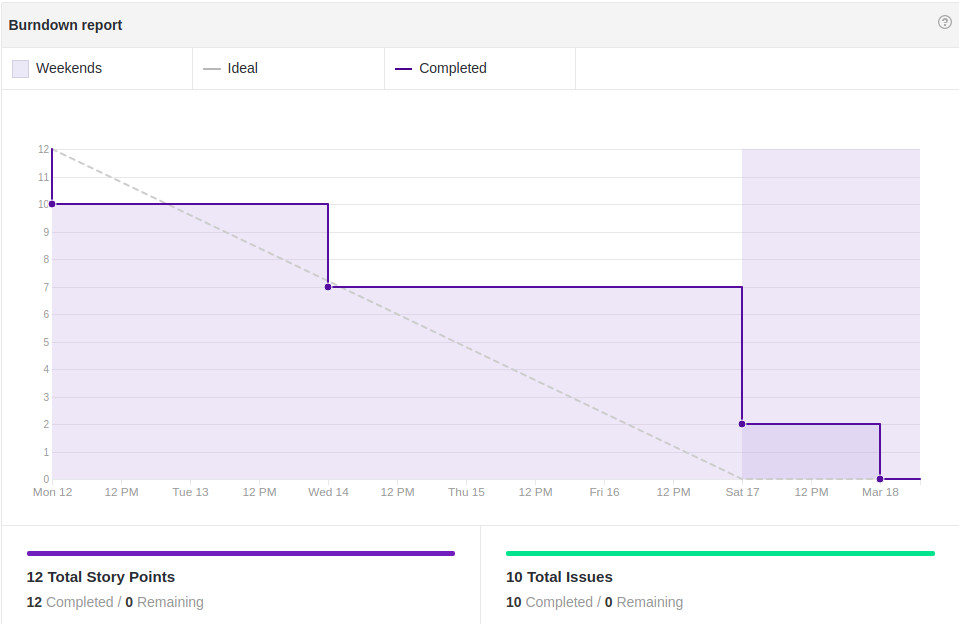
\includegraphics[width=\textwidth]{burn3.jpg}
    \caption{Burndown Chart Sprint 3}
    \label{fig:burn3}
\end{figure}

\newpage
\section{Sprint 4 - Fancy Quizes and Defect Fixing}
\subsection{Sprint Planning}
This sprint focused on addressing a critial bug in the production environment
concerning the PDF to PNG conversion. Extra types of quizzes would also be added
to complement the single choice ones available at the moment. The entire list of estimated stories
can be found in the \autoref{chap:spintstories} of this report.

\subsection{Production Environment Bug}
The presentation file upload and splitting of slides into PNG images persisted
together with text implemented in sprint 2, worked as expected in both development and testing environments.
The production environment on the other hand, would randomly crash and the underlying cause had
to be investigated before any other work could progress. The process of splitting the
PDF presentations uploaded relied on splitting the intial file into separate, single
paged PDF files, extracting their text, converting them to PNG images, before grouping
together and persisting in the database. The final part of asynchronously trying
to convert single paged PDF files into PNG files, failed with an IO exception, where
the underlying PDFtk\cite{55} command line utility could not find a PDF file, even though it was
there.

\begin{figure}[h!]
    \centering
    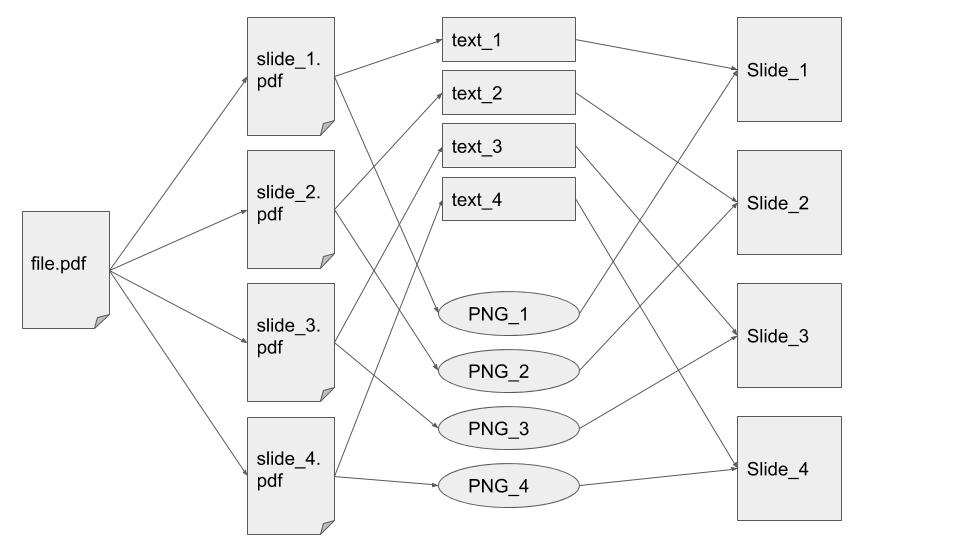
\includegraphics[width=0.8\textwidth]{split1.jpg}
    \caption{Initial Slide Extraction}
    \label{fig:split1}
\end{figure}

\newpage
My initial thought was that the problem was due to a race condition, where asynchronous
code was trying to get access to the file system. This would mean the code worked as expected
on my much more powerful laptop only by luck. Making the algorithm to process
files synchronously, did fix the problem for smaller PDF presentations, however attempting
to upload a larger test PDF crashed the production environment in the same manner.
Finally, the algorithm has been changed to no longer use single paged PDFs, and convert them
one by one to PNGs. The scissors library has been removed, and the node-pdf2img\cite{56} used
instead to take the whole PDF presentation, and extract all the PNG files from it using a
single PDFtk call. The algorithm could stay asynchronous, and the file system access has been almost halved.

\begin{figure}[h!]
    \centering
    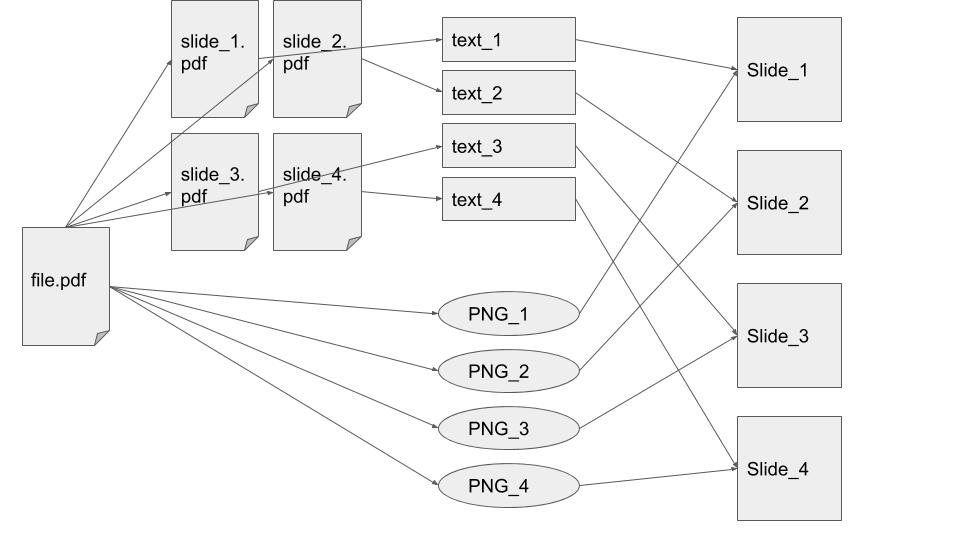
\includegraphics[width=0.8\textwidth]{split2.jpg}
    \caption{Final Slide Extraction}
    \label{fig:split2}
\end{figure}

\newpage
\subsection{Extra Types of Quizzes}
The \texttt{isQuiz} boolean flag was no longer appropriate if extra types of quizzes were
to be supported. Every slide could be made into a true/false quiz, and quizzes eligible
to become single choice, could also be marked as multi choice. Changing the slide eligibility
algorithm was the first step towards having support for all three quizzes. The initial version
checked if slide's text contained at least "A)" and "B)". The improved version would make a
slide eligible to become a quiz if one of the following was true:

\begin{itemize}
  \item "A)" and "B)" was found in the slide's text
  \item "A." and "B." was found in the slide's text
  \item At least two bullet characters were found
\end{itemize}

The \texttt{isQuiz} flag of the \texttt{Slide} schema object has been changed to a \texttt{quizType}
of type \texttt{string}. It could take the value of \texttt{null}, \texttt{"truefalse"}, \texttt{"single"}
and \texttt{"multi"}. Furthermore, the JSON message bundled with the \texttt{slide-change} Socket.io
event was changed to:

\begin{figure}[h!]
  \begin{lstlisting}[basicstyle=\small]
  {
    "img": "base64encodedImage",
    "text": "textOfTheSlide"
    "quizType": "truefalse"
    "sessionCode": "ABCD1234"
  }
  \end{lstlisting}
  \caption{The Final JSON Message Broadcasted on Slide Change}
\end{figure}

This enabled the student's client to know how to render the quiz appropriately. For example if
the current slide was marked as a multi choice, the client would use the text of the slide,
extract the answers buttons e.g. "A", "B" and "C", and let student submit their answer.
The answer could no longer be a single option. It was therefore changed to an array of options.

\begin{figure}[h!]
  \begin{lstlisting}[basicstyle=\small]
  {
    "sessionCode": "ABCD1234",
    "options": ["A", "C"]
  }
  \end{lstlisting}
  \caption{The Final JSON Message Emitted when Student Submitted his Answer}
\end{figure}

\subsection{Sprint Retrospective}
Following this sprint, the Quiz Tool was almost complete. The persistence and report
generation was still missing, but the core functionality including the ability
to add various quizzes into slides, and broadcast them to students was finished.
The full sprint retrospective document produced can be found in the
\autoref{chap:spintretrospectives} of this report.

\begin{figure}[h!]
    \centering
    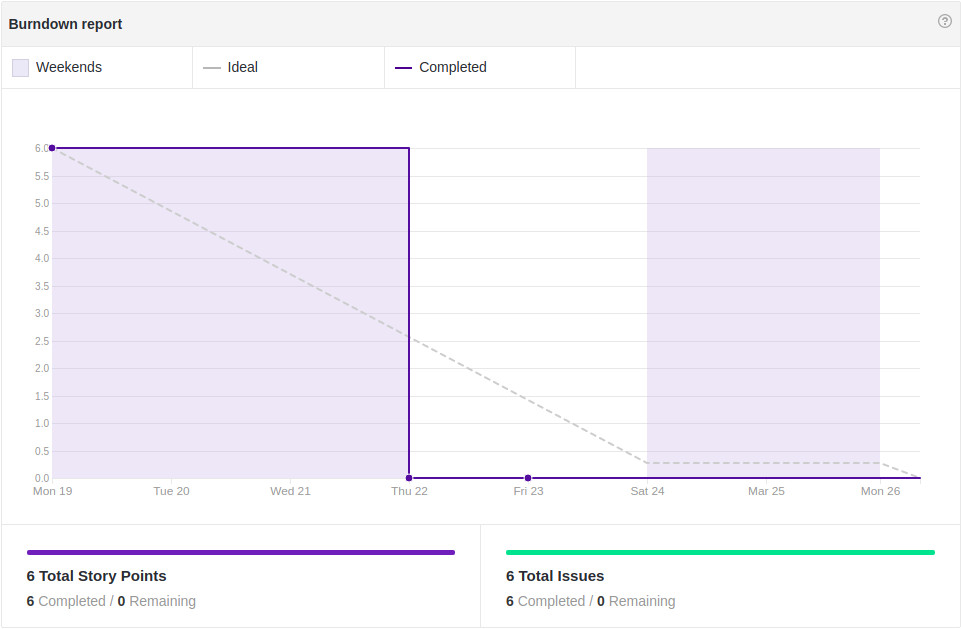
\includegraphics[width=\textwidth]{burn4.jpg}
    \caption{Burndown Chart Sprint 4}
    \label{fig:burn4}
\end{figure}

\section{Sprint 5 - Persistence, Report Generation and Testing}
\subsection{Sprint Planning}
The final sprint focused on the persistence of students' answers in the database and
generation of PDF reports based on these answers. User friendly error handler has
also been added, and the application has been polished before the Quiz Tool implementation
was over. As always, the entire list of estimated stories
can be found in the \autoref{chap:spintstories} of this report.

\subsection{Database Container Persistence}
Docker containers do not persist data by design. Every time the \texttt{database}
container has been brought up and down, by both docker-compose and the
Milticontainer Elastic Beanstalk environment, any data stored in the MongoDB
would be lost. This behaviour is perfect for running tests, where the starting
environment is expected to be the same between tests. It was however unacceptable
for the production environment.

The \texttt{Dockerrun.aws.json} file included in the \autoref{chap:codesamples} of this report
as the \autoref{sample:dockerrunawsfinal}, shows the final configuration of the production
environment running on AWS. The volume mount called "mongo" has been added, which maps the
\texttt{/data/db} directory in the \texttt{database} container onto the \texttt{/var/app/database}
directory on the underlying EC2 instance running the container cluster. This causes the database
to persist its data even when the application is re-deployed. The only time the data could
be lost, is when the EC2 instance is destroyed, when for example more RAM has been requested
for the environment.

\subsection{Lecture Answers Persistence}

\subsection{Report Generataion}


\subsection{Sprint Retrospective}
The full sprint retrospective document produced can be found in the
\autoref{chap:spintretrospectives} of this report.

\chapter{Final Design}

This chapter follows on the discussion of the individual sprints and summarises
the final design of the tool.

\chapter{Testing}

\section{Server Side Unit Tests}
\section{Client Side Unit Tests}
\section{Selenium Integration Tests}

% You should concentrate on the more important aspects of the design. It is essential that an overview is presented before going into detail. As well as describing the design adopted it must also explain what other designs were considered and why they were rejected.
%
% The design should describe what you expected to do, and might also explain areas that you had to revise after some investigation.
%
% Typically, for an object-oriented design, the discussion will focus on the choice of objects and classes and the allocation of methods to classes. The use made of reusable components should be described and their source referenced. Particularly important decisions concerning data structures usually affect the architecture of a system and so should be described here.
%
% How much material you include on detailed design and implementation will depend very much on the nature of the project. It should not be padded out. Think about the significant aspects of your system. For example, describe the design of the user interface if it is a critical aspect of your system, or provide detail about methods and data structures that are not trivial. Do not spend time on long lists of trivial items and repetitive descriptions. If in doubt about what is appropriate, speak to your supervisor.
%
% You should also identify any support tools that you used. You should discuss your choice of implementation tools - programming language, compilers, database management system, program development environment, etc.
%
% Some example sub-sections may be as follows, but the specific sections are for you to define.

% \section{Overall Architecture}
%
% \section{Some detailed design}
%
% \subsection{Even more detail}
%
% \section{User Interface}
%
% \section{Other relevant sections}

% \chapter{Implementation}
% The implementation should look at any issues you encountered as you tried to implement your
% design. During the work, you might have found that elements of your design were unnecessary or
% overly complex; perhaps third party libraries were available that simplified some of the functions
% that you intended to implement. If things were easier in some areas, then how did you adapt your
% project to take account of your findings?
% It is more likely that things were more complex than you first thought. In particular, were there
% any problems or difficulties that you found during implementation that you had to address? Did
% such problems simply delay you or were they more significant?
% You can conclude this section by reviewing the end of the implementation stage against the
% planned requirements

% \chapter{Testing}
%
% Detailed descriptions of every test case are definitely not what is required here. What is important is to show that you adopted a sensible strategy that was, in principle, capable of testing the system adequately even if you did not have the time to test the system fully.
%
% Provide information in the body of your report and the appendix to explain the testing that has been performed. How does this testing address the requirements and design for the project?
%
% How comprehensive is the testing within the constraints of the project?  Are you testing the normal working behaviour? Are you testing the exceptional behaviour, e.g. error conditions? Are you testing security issues if they are relevant for your project?
%
% Have you tested your system on ``real users''? For example, if your system is supposed to solve a problem for a business, then it would be appropriate to present your approach to involve the users in the testing process and to record the results that you obtained. Depending on the level of detail, it is likely that you would put any detailed results in an appendix.
%
% The following sections indicate some areas you might include. Other sections may be more appropriate to your project.

% \section{Overall Approach to Testing}
%
% \section{Automated Testing}
%
% \subsection{Unit Tests}
%
% \subsection{User Interface Testing}
%
% \subsection{Stress Testing}
%
% \subsection{Other types of testing}
%
% \section{Integration Testing}
%
% \section{User Testing}

\chapter{Evaluation}

Examiners expect to find in your dissertation a section addressing such questions as:

\begin{itemize}
   \item Were the requirements correctly identified? 
   \item Were the design decisions correct?
   \item Could a more suitable set of tools have been chosen?
   \item How well did the software meet the needs of those who were expecting to use it?
   \item How well were any other project aims achieved?
   \item If you were starting again, what would you do differently?
\end{itemize}

Other questions can be addressed as appropriate for a project. 

Such material is regarded as an important part of the dissertation; it should demonstrate that you are capable not only of carrying out a piece of work but also of thinking critically about how you did it and how you might have done it better. This is seen as an important part of an honours degree. 

There will be good things and room for improvement with any project. As you write this section, identify and discuss the parts of the work that went well and also consider ways in which the work could be improved. 

In the latter stages of the module, we will discuss the evaluation. That will probably be around week 9, although that differs each year. 
% add any additional chapters here

\setemptyheader
\addcontentsline{toc}{chapter}{Appendices}
\chapter*{Appendices}
The appendices are for additional content that is useful to support the discussion in the report. It is material that is not necessarily needed in the body of the report, but its inclusion in the appendices makes it easy to access.

For example, if you have developed a Design Specification document as part of a plan-driven approach for the project, then it would be appropriate to include that document as an appendix. In the body of your report you would highlight the most interesting aspects of the design, referring your reader to the full specification for further detail.

If you have taken an agile approach to developing the project, then you may be less likely to have developed a full requirements specification. Perhaps you use stories to keep track of the functionality and the 'future conversations'. It might not be relevant to include all of those in the body of your report. Instead, you might include those in an appendix.

There is a balance to be struck between what is relevant to include in the body of your report and whether additional supporting evidence is appropriate in the appendices. Speak to your supervisor or the module coordinator if you have questions about this.

\pagebreak

% start the appendix - sets up different numbering
\fancypagestyle{plain}{%
%\fancyhf{} % clear all header and footer fields
\fancyhead[L]{\textsl{Appendix\ \thechapter}}
\fancyhead[R]{\textsl{\leftmark}}}

\appendix
\fancyhead[L]{\textsl{Appendix\ \thechapter}}
\fancyhead[R]{\textsl{\leftmark}}
\fancyhead[C]{}
\fancyfoot[C]{\thepage}
\renewcommand{\headrulewidth}{0.4pt}
\renewcommand{\chaptermark}[1]{\markboth{#1}{}}

\fancyhead[L]{\textsl{Appendix\ \thechapter}}
\fancyhead[R]{\textsl{\leftmark}}
\fancyfoot[C]{{\thepage} of \pageref{LastPage}}

% include any appendices here
\chapter{Third-Party Code and Libraries}
%
% If you have made use of any third party code or software libraries, i.e. any code
% that you have not designed and written yourself, then you must include this appendix.
%
% As has been said in lectures, it is acceptable and likely that you will make use of
%  third-party code and software libraries. If third party code or libraries are used,
%   your work will build on that to produce notable new work. The key requirement is that we
%   understand what is your original work and what work is based on that of other people.
%
% Therefore, you need to clearly state what you have used and where the original material can be
% found. Also, if you have made any changes to the original versions, you must explain what you have changed.
%
% As an example, you might include a definition such as:
%
% Apache POI library - The project has been used to read and write Microsoft Excel files (XLS) as
%  part of the interaction with the client's existing system for processing data. Version 3.10-FINAL
%   was used. The library is open source and it is available from the Apache Software Foundation
% \cite{apache_poi}. The library is released using the Apache License
% \cite{apache_license}. This library was used without modification.

% server package.json
\subparagraph{body-parser v1.18.2}
MIT licensed Node.js middleware for parsing bodies of incoming HTTP requests. Used as part of the
\texttt{server\_node} container. [Online] Available: https://github.com/expressjs/body-parser, [Accessed: Apr. 20, 2018].

\subparagraph{express v4.15.2}
MIT licensed Node.js web development framework used to develop the back end of the Quiz Tool.
[Online] Available: https://github.com/expressjs/body-parser, [Accessed: Apr. 20, 2018].

\subparagraph{eyes v0.1.8}

\subparagraph{fs v0.0.1-security}
\subparagraph{jsonschema v1.2.2}
\subparagraph{mongoose v5.0.7}
\subparagraph{multer v1.3.0}
\subparagraph{passport v0.4.0}
\subparagraph{passport-google-oauth v1.0.0}
\subparagraph{pdf-extract v1.0.11}
\subparagraph{pdf2img v0.5.0}
\subparagraph{request-promise v4.2.2}
\subparagraph{request v2.83.0}
\subparagraph{socket.io v2.0.4}
\subparagraph{mocha v5.0.4}
\subparagraph{chai v4.1.2}
\subparagraph{chai-http v3.0.0}
\subparagraph{selenium-webdriver v4.0.0-alpha.1}

% server Dockerfile
\subparagraph{ghostscript}
\subparagraph{poppler-utils}
\subparagraph{pdftk}
\subparagraph{graphicsmagick}

% client package.json
\subparagraph{@angular/animations v4.4.4}
\subparagraph{@angular/common v4.3.5}
\subparagraph{@angular/compiler v4.3.5}
\subparagraph{@angular/core v4.3.5}
\subparagraph{@angular/forms v4.3.5}
\subparagraph{@angular/http v4.3.5}
\subparagraph{@angular/platform-browser v4.3.5}
\subparagraph{@angular/platform-browser-dynamic v4.3.5}
\subparagraph{@angular/router v4.3.5}
\subparagraph{@types/jspdf v1.1.31}
\subparagraph{@types/socket.io-client v1.4.32}
\subparagraph{chart.js v2.7.2}
\subparagraph{file-saver v1.3.8}
\subparagraph{core-js v2.5.0}
\subparagraph{font-awesome v4.7.0}
\subparagraph{intl v1.2.5}
\subparagraph{jspdf v1.3.5}
\subparagraph{jspdf-autotable v2.3.2}
\subparagraph{mdi v2.1.19}
\subparagraph{ng2-charts v1.6.0}
\subparagraph{ng2-file-upload v1.3.0}
\subparagraph{ng2-materialize v1.8.0}
\subparagraph{ngx-cookie-service v1.0.10}
\subparagraph{rxjs v5.4.3}
\subparagraph{socket.io-client v2.0.4}
\subparagraph{zone.js v0.8.16}
\subparagraph{@angular/cli v1.3.1}
\subparagraph{@angular/compiler-cli v4.3.5}
\subparagraph{@types/jasmine v2.5.38}
\subparagraph{codelyzer v3.1.2}
\subparagraph{jasmine-core v2.5.2}
\subparagraph{jasmine-spec-reporter v3.2.0}
\subparagraph{karma v1.4.1}
\subparagraph{karma-cli v1.0.1}
\subparagraph{karma-coverage-istanbul-reporter v0.2.0}
\subparagraph{karma-jasmine v1.1.0}
\subparagraph{karma-jasmine-html-reporter v0.2.2}
\subparagraph{karma-phantomjs-launcher v1.0.4}
\subparagraph{protractor v5.1.0}
\subparagraph{ts-node v3.3.0}
\subparagraph{tslint v5.6.0}
\subparagraph{typescript v2.4.2}

% tutorials
\subparagraph{Building Chat Application using MEAN Stack (Angular 4) and Socket.io}
Step by step tutorial of building a simple chat application using MEAN stack and Socket.io. It helped me
to understand how to use MEAN with Socket.io together, and the initial structure of the application
was inspired by it.
[Online] Available: https://www.djamware.com/post/58e0d15280aca75cdc948e4e/building-chat-applicationusing-mean-stack-angular-4-and-socketio,
[Accessed: Apr. 11, 2018].

\subparagraph{Docker Compose | Containerizing MEAN Stack Application | DevOps Tutorial | Edureka}
A YouTube tutorial explaining how to containerise a MEAN stack web application. The \texttt{docker-compose.yml}
file has been based on the one showed in the video. [Online] Available: https://www.youtube.com/watch?v=WZa7GsqyS3w,
[Accessed: Apr. 20, 2018].

\subparagraph{Dockerized Angular 4 App (with Angular CLI)}
MIT licensed GitHub repository showing a starter Angular application, containerised with nginx
using Docker. The structure of \texttt{client} container is based on a fork of the repository.
[Online] Available: https://github.com/avatsaev/angular4-docker-example, [Accessed: Apr. 20, 2018].

\subparagraph{Multicontainer Docker Environments}
An official AWS tutorial showing how to deploy an application to the Multicontainer Elasticbeanstalk Docker
Environment. [Online] Available: https://docs.aws.amazon.com/elasticbeanstalk/latest/dg/create\_deploy\_docker\_ecs.html, [Accessed: Apr. 20, 2018].

\subparagraph{Test a Node RESTful API with Mocha and Chai}
A tutorial showing how to tests Node.js applications with Mocha and Chai. The structure of the server side
unit tests has been inspired by the tutorial. [Online] Available: https://scotch.io/tutorials/test-a-node-restful-api-with-mocha-and-chai,
[Accessed: Apr. 20, 2018].

\subparagraph{MEAN with Angular 2/5 - User Registration and Login Example \& Tutorial}
The authentication of the Quiz Tool has been inspired by this tutorial. Especially the Angular
JWT interceptor used in the application to append authentication tokens to each HTTP requests is based on the
code presented in the tutorial. [Online] Available: http://jasonwatmore.com/post/2017/02/22/mean-with-angular-2-user-registration-and-login-example-tutorial,
[Accessed: Apr. 20, 2018].

\subparagraph{6 16 integrating with google oauth with passport js in a MEAN app undergrad webdev summer 1 2017}
A YouTube tutorial explaining how to configure google authentication with the passport Node.js
authentication middleware, in a MEAN stack application. The Google Sign-In implemented in Quiz Tool
has been based on this tutorial. [Online] Available: https://www.youtube.com/watch?v=rc6zYV4jShQ,
[Accessed: Apr. 20, 2018].

\subparagraph{How to setup Elastic Beanstalk Deployment?}
A topic in the official Circle CI discussion forum describing how to setup Circle CI to automatically
deploy to the Elastic Beanstalk environment hosted on AWS. [Online] Available: https://discuss.circleci.com/t/how-to-setup-elastic-beanstalk-deployment/6154/4,
[Accessed: Apr. 20, 2018].

\subparagraph{Getting Started with Docker Compose}
A step-by-step introduction to using the official Selenium Docker images using docker-compose. The tutorial
was used when integration selenium tests were added to test the application.
[Online] Available: https://github.com/SeleniumHQ/docker-selenium/wiki/Getting-Started-with-Docker-Compose,
[Accessed: Apr. 20, 2018].










%


\chapter{Ethics Submission}

Ethics Application Number: 9624

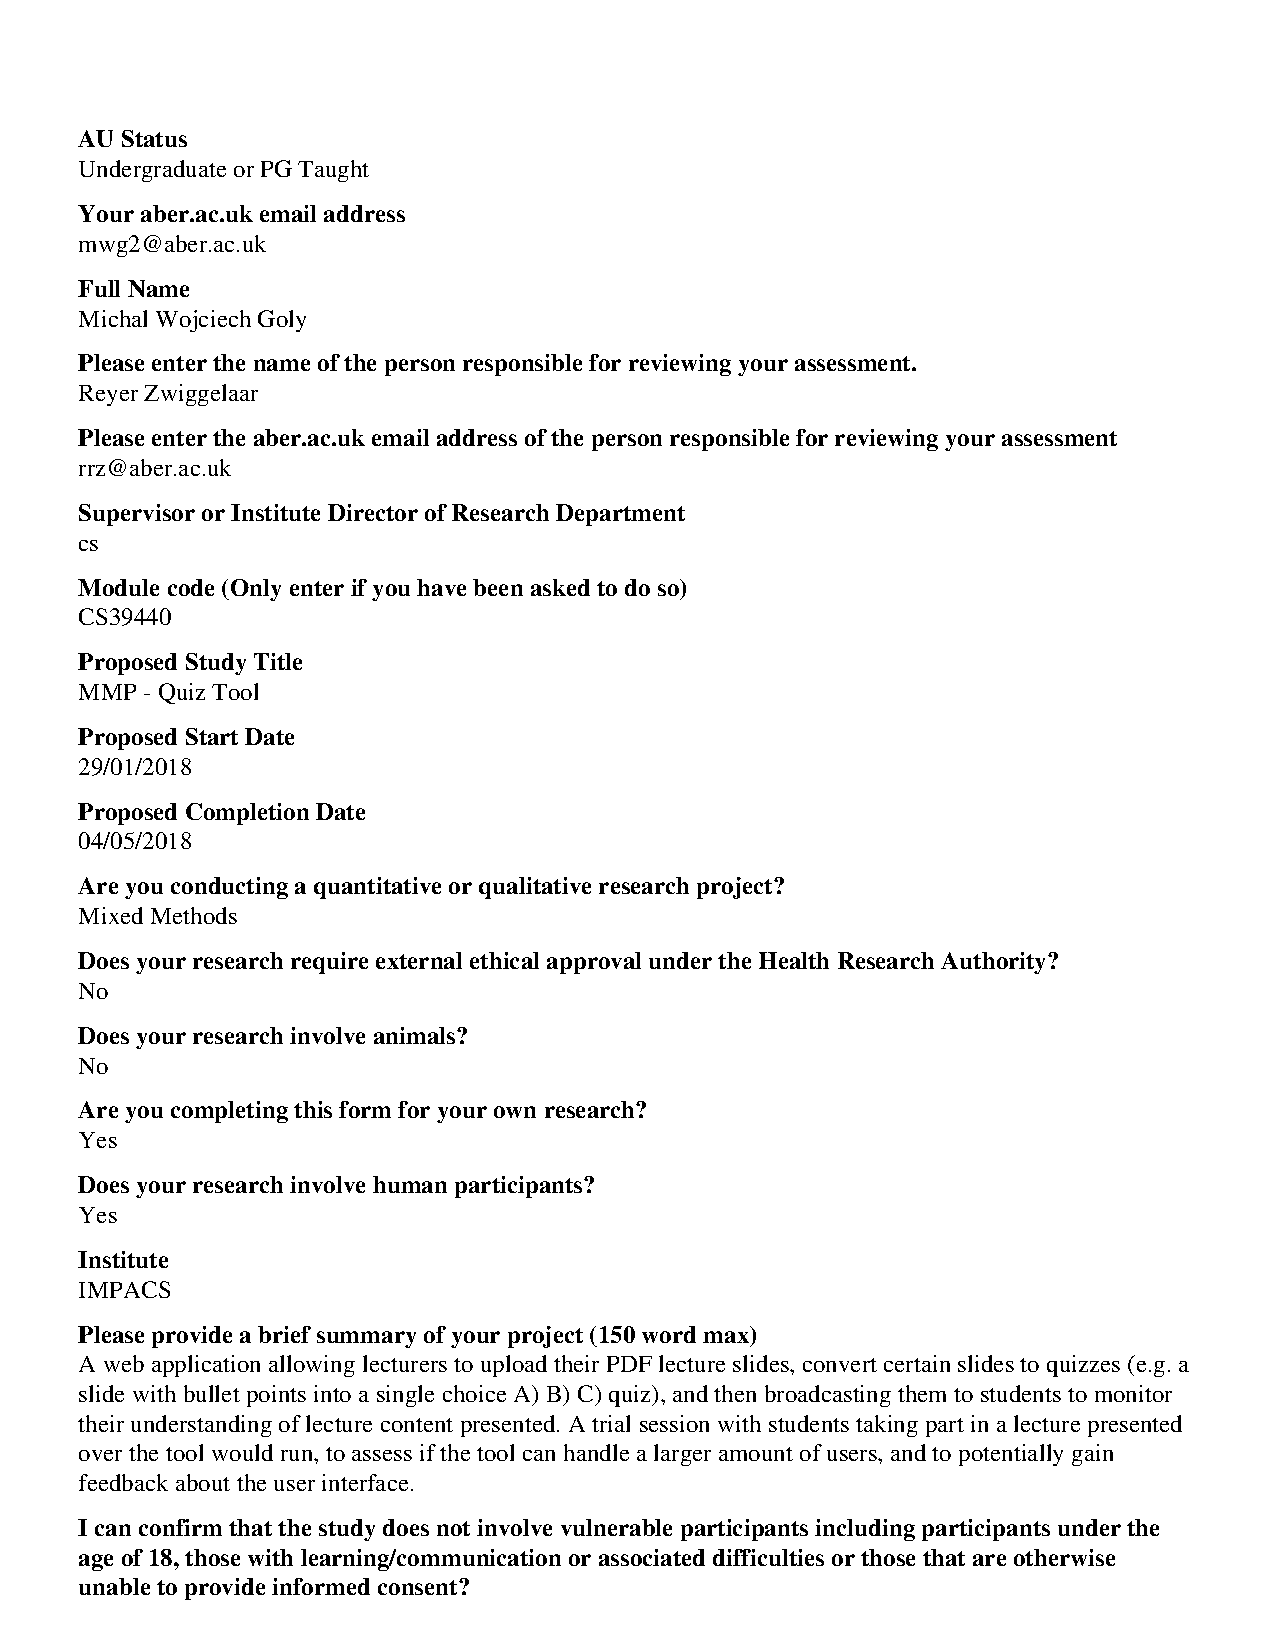
\includepdf[pages=-]{Appendix2/9624.pdf}

\chapter{Sprint Stories}
\label{chap:spintstories}

This appendix contains the user stories produced before each sprint. 

\section{Sprint 1}
\begin{figure}[ht]
    \centering
    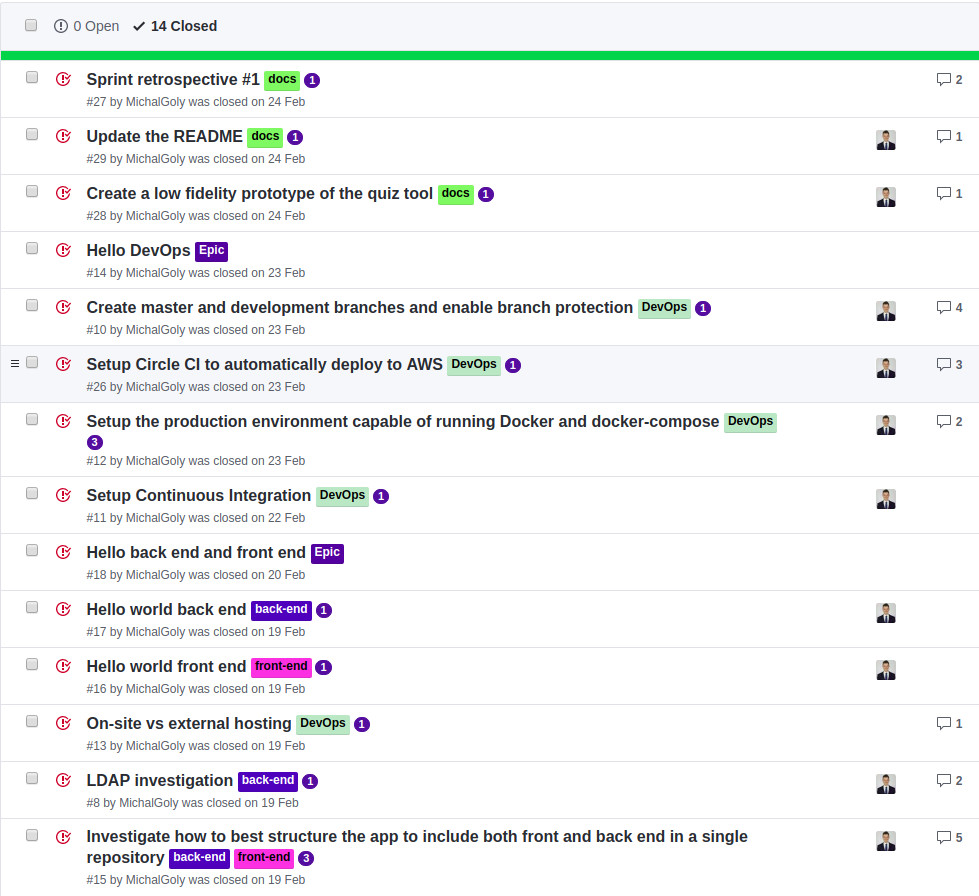
\includegraphics[width=0.9\textwidth]{Appendix3/1.jpg}
    \caption{Stories Sprint 1}
    \label{fig:sprintstories1}
\end{figure}

\section{Sprint 2}
\section{Sprint 3}
\section{Sprint 4}
\section{Sprint 5}


\fancypagestyle{plain}{%
   \fancyhead{} %[C]{Annotated Bibliography}
   \fancyfoot[C]{{\thepage} of \pageref{LastPage}} % except the center
   \renewcommand{\headrulewidth}{0pt}
   \renewcommand{\footrulewidth}{0pt}
}

\setemptyheader

% the following line is included so that the bibliography is also shown in the table of contents. There is the possibility that this is added to the previous page for the bibliography. To address this, a newline is added so that it appears on the first page for the bibliography.
\addcontentsline{toc}{chapter}{Bibliography} % Adds References to contents page

\begin{thebibliography}{1}

\bibitem{1} Qwizdom, “Qwizdom homepage,” 2018. [Online] Available: https://qwizdom.com/, [Accessed: Apr. 9, 2018].

  Qwizdom is the tool currently used by the univeristy and will be replaced with this project.

\bibitem{2} Google Sign-In, "Google Identity homepage", 2018. [Online] Available: https://developers.google.com/identity/, [Accessed: Apr. 10, 2018].

  Google Sign-In is a secure authentication system that reduces the burden of login for your users, by enabling them
  to sign in with their Google account. The same account they already use with Gmail, Play, Google+, and other Google services.

\bibitem{3} Java Programming Language, "Java homepage", 2018. [Online] Available:
  https://docs.oracle.com/javase/8/docs/technotes/guides/language/index.html, [Accessed: Apr. 11, 2018].

  The Java™ Programming Language is a general-purpose, concurrent, strongly typed, class-based object-oriented language.
  It is normally compiled to the bytecode instruction set and binary format defined in the Java Virtual Machine Specification.

\bibitem{4} Android, "Android homepage", 2018. [Online] Available: https://www.android.com/, [Accessed: Apr. 11, 2018].

  Android is a mobile operating system developed by Google.

\bibitem{5} iOS, "Apple homepage", 2018. [Online] Available: https://www.apple.com/uk/ios/ios-11/, [Accessed: Apr. 11, 2018].

  iOS is a mobile operating system created and developed by Apple Inc.

\bibitem{6} React Native, "React Native homepage", 2018. [Online] Available: https://facebook.github.io/react-native/, [Accessed: Apr. 11, 2018].

  React Native lets you build mobile apps for both iOS and Android using only JavaScript.

\bibitem{7} JavaScript Programming Language, "JavaScript Mozilla docs", 2018. [Online]
  Available: https://developer.mozilla.org/bm/docs/Web/JavaScript, [Accessed: Apr. 11, 2018].

  JavaScript is a lightweight, interpreted, programming language, best known for being the scripting
  language of the web.

\bibitem{8} React, "React homepage", 2018. [Online] Available: https://reactjs.org/, [Accessed: Apr. 11, 2018].

  A JavaScript library for building user interfaces.

\bibitem{9} Angular, "Angular homepage", 2018. [Online] Available: https://angular.io/, [Accessed: Apr. 11, 2018].

  Angular is a TypeScript-based front end development framework supported by Google.

\bibitem{10} TypeScript Programming Language, "TypeScript homepage", 2018. [Online] Available: https://www.typescriptlang.org/, [Accessed: Apr. 11, 2018].

  TypeScript is a typed superset of JavaScript that compiles to plain JavaScript.

\bibitem{11} I. Fette, A. Melnikov, "The WebSocket Protocol", [Online] Available: https://tools.ietf.org/html/rfc6455, [Accessed: Apr. 11, 2018].

  The WebSocket Protocol enables two-way communication between a client running untrusted code in a controlled environment to a remote host
  that has opted-in to communications from that code.

\end{thebibliography}

\end{document}
